\chapter{航天器姿态运动学}
\thispagestyle{empty}

\section{航天器常用坐标系}
\subsection{基本概念}
\vspace*{-1em}

\defination[天体坐标系基本概念]
{
	\dy[天球]{{\text{T}}Q}\quad 指一个以地球质心$M$为中心,半径$r$为任意长的一个假想的球体 。其目的是将天体沿观测者视线投影到球面上,以便于研究天体及其相互关系。\\
	\hspace*{2.2em}\dy[黄道平面]{HDPM}\quad 由于地球绕太阳公公转而产生的,即地球公转轨道在天球上的反映称为黄道。它和赤道面相交于春分点和秋分点。\\
	\hspace*{2.2em}\dy[春分点]{CFD}\quad 指太阳从难向北在黄赤道上的交点。
}

\begin{figure}[!htb]
	\begin{minipage}{0.45\linewidth}
		\centering
		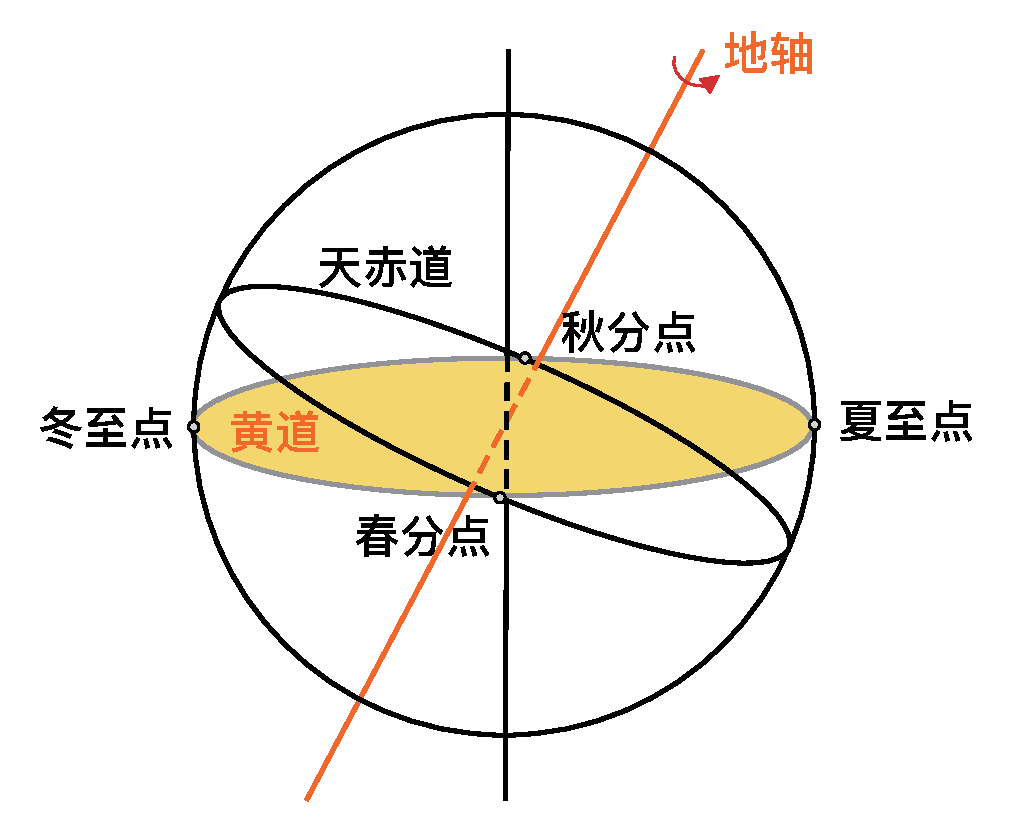
\includegraphics[width=\linewidth]{pic/基本概念}
		\caption{天球坐标系的基本概念}
		\label{基本概念}
	\end{minipage}
	\begin{minipage}{0.55\linewidth}
		\centering
		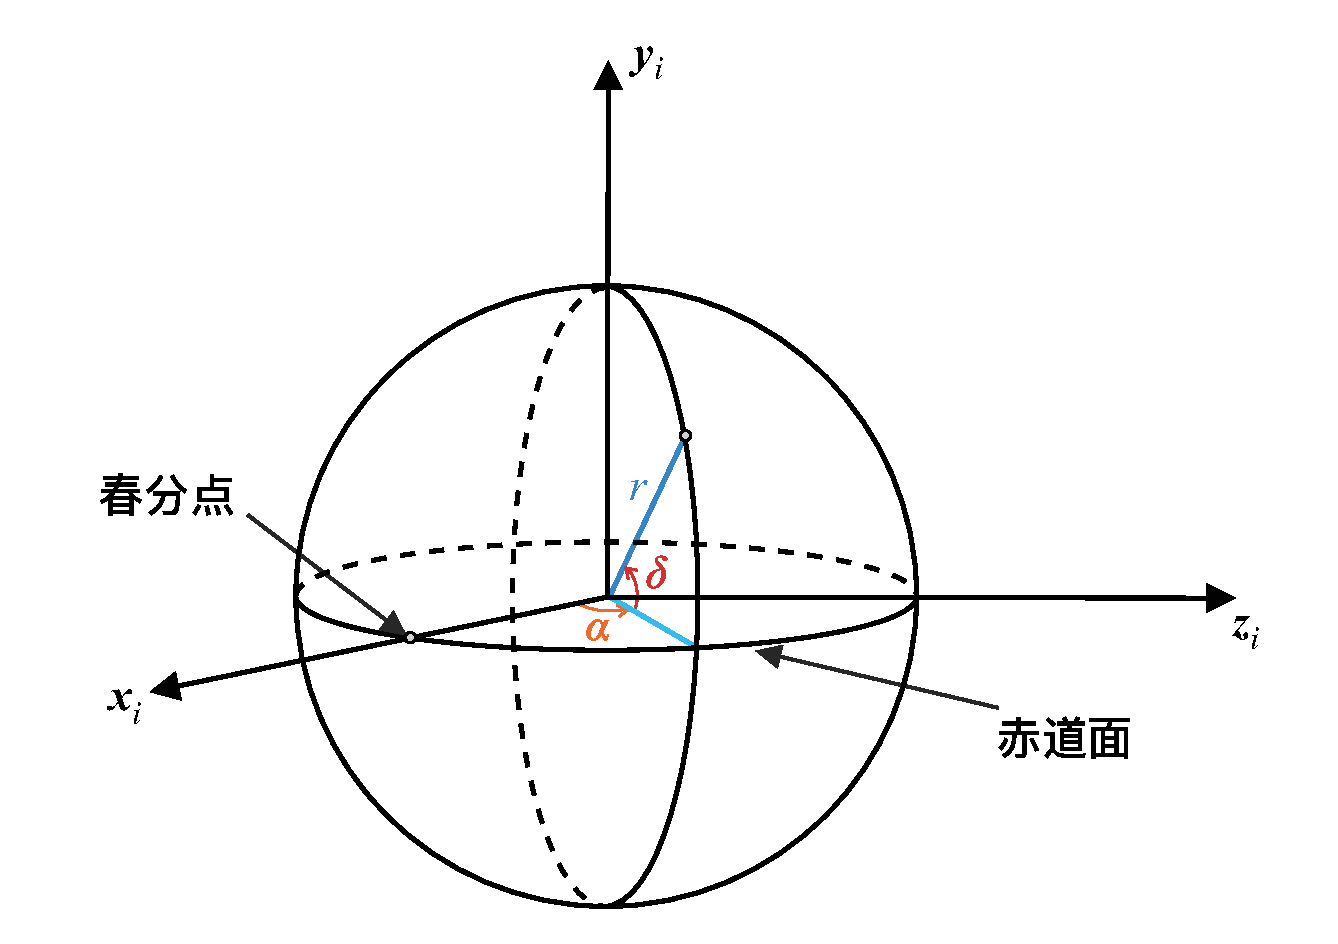
\includegraphics[width=\linewidth]{pic/地惯}
		\vspace*{-2.95em}
		\caption{地心赤道惯性坐标系}
		\label{地惯}
	\end{minipage}
\end{figure}


\subsection{地心赤道惯性坐标系}
\vspace*{-1em}

\defination[地心赤道惯性坐标系]
{
	如图 \ref{地惯} 所示,\dy[地心第一赤道坐标系]{DXDYCDZBX},简称为\dy[惯性坐标系]{GXZBX}。$X$轴在地球赤道平面内,指向赤道平面与黄道平面的相交线交点(春分点)。$Z$轴垂直于赤道平面,与地球自转角速度矢量方向一致。J2000的地心平赤道、平春分点的地心赤道坐标系。
}


\subsection{地心赤道旋转坐标系}
\vspace*{-1em}

\defination[地心赤道坐标系]
{
	如图 \ref{地心旋转} 所示,\dy[地心赤道旋转坐标系]{DXCDXZZBX},也叫\dy[地心第四赤道坐标系]{DXDSCDZBX}。$X$轴在赤道平面内,指向\dy[格林威治子午线]{GLNZZWX},$Z$轴垂直于赤道平面,与地球自转角速度矢量方向一致。$\lambda$是地理经度,从格林威治子午线向东度量,$\phi$是地心纬度。
}
\nomenclature{$\lambda$}{地理经度 \nomrefpage}
\nomenclature{$\phi$}{地理纬度 \nomrefpage}

\begin{figure}[!htb]
	\begin{minipage}{0.485\linewidth}
		\centering
		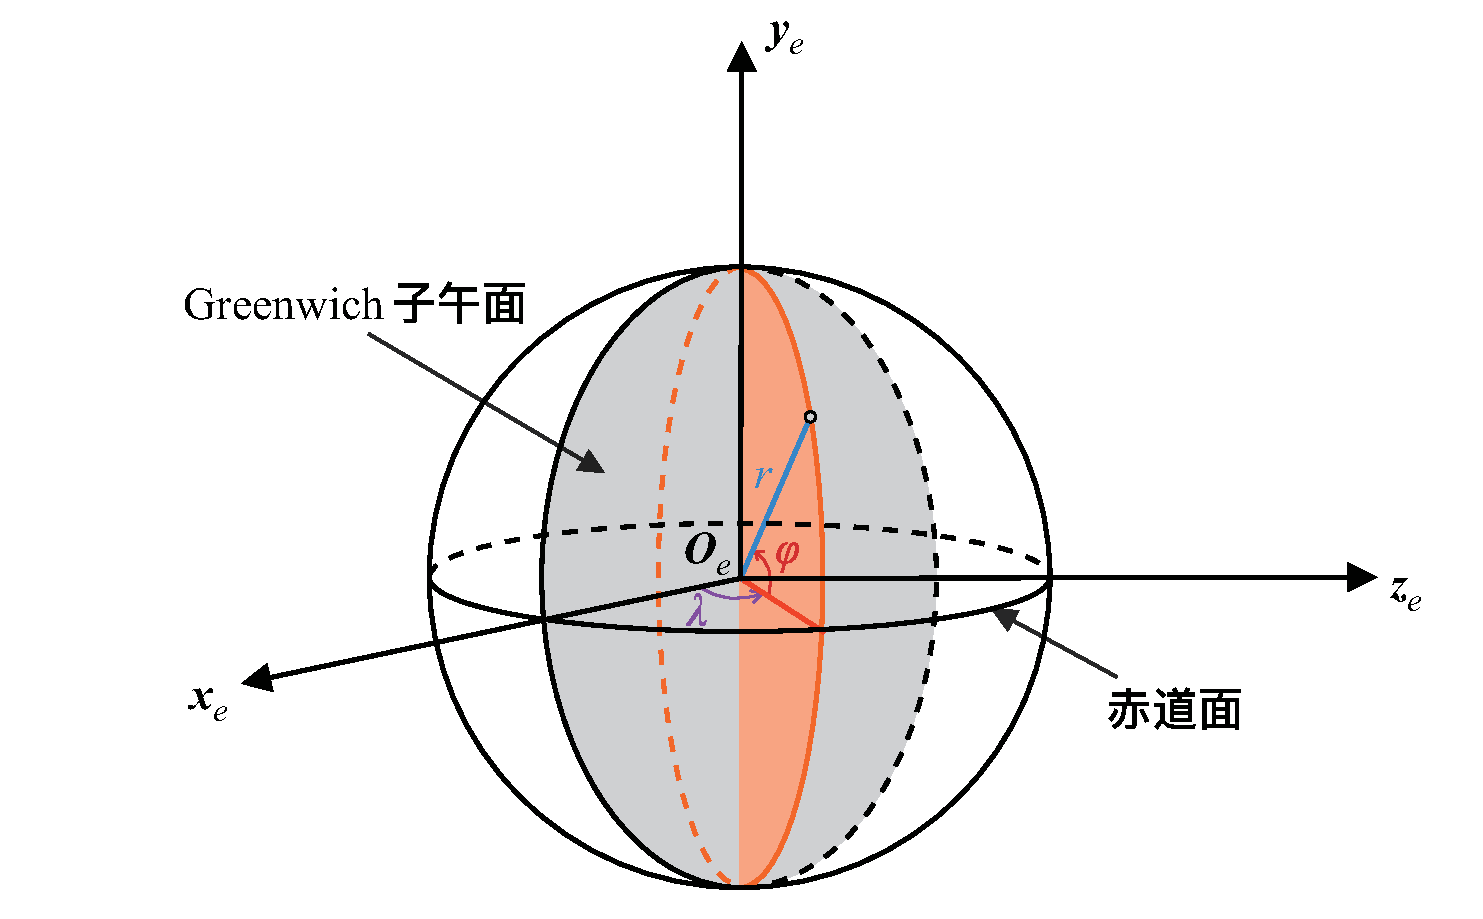
\includegraphics[width=\linewidth]{pic/地心旋转}
		\caption{地心赤道旋转坐标系}
		\label{地心旋转}
	\end{minipage}
	\begin{minipage}{0.515\linewidth}
		\centering
		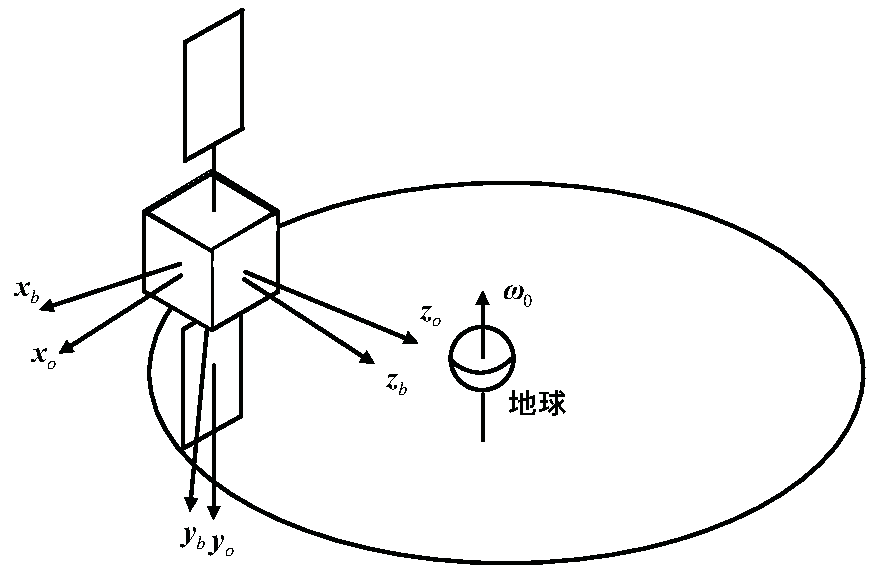
\includegraphics[width=\linewidth]{pic/轨道星体}
		\caption{轨道坐标系和星体坐标系}
		\label{轨道星体}
	\end{minipage}
\end{figure}


\subsection{轨道坐标系和星体坐标系}
\vspace*{-1em}

\defination[地心赤道坐标系]
{
	\dy[轨道坐标系]{DY}\quad 原点在飞行器质心,$z_o$轴指向地心,$x_o$轴在轨道面内与$z_o$轴垂直,指向速度方向,$y_o$轴在轨道平面法线方向,与$x_o$,$z_o$轴成右手正交坐标系。\\
	\hspace*{2.2em}\dy[星体坐标系]{X{\text{T}}ZBX}\quad 原点在质心,$x_b$轴为\dy[滚动轴]{GDZ},$y_b$轴为\dy[俯仰轴]{FYZ},$z_b$轴为\dy[偏航轴]{PHZ}。(对地定向航天器)
}


\section{姿态参数}
\subsection{向量的描述及向量运算的矩阵表示}
对于任意一个\dy[向量]{XL}$\bm{u}$,都可以表示为某个\dy[向量基]{XLJ}
$\underline{\bm{e}} = \big[ \bm{i} \quad \bm{j} \quad \bm{k} \big]^\T $的\dy[基向量]{JXL}的线性组合,即
\begin{equation}
	\bm{u} = u_s \bm{i} + u_y \bm{j} + u_z \bm{k}
	\nomenclature{$\bm{u}$}{三维向量$\bm{u}$\nomrefpage}
	\nomenclature{$\ubm{e}$}{三维向量基$\ubm{e}$\nomrefpage}
	\nomenclature{$\underline{\bm{u}}$}{三维向量$\bm{u}$的分量矩阵,用于向量的矩阵运算,为了将向量和矩阵区别,后文中的矩阵均加了下划线\nomrefpage}
\end{equation}
其中,$\bm{i}, \bm{j}, \bm{k}$分别称为向量$\bm{u}$在基向量上的3个分向量,3个标量系数$u_x,u_y,u_z$分别称为向量$\bm{u}$在3个基向量上的坐标。这3个坐标构成一个标量矩阵,称为向量$\bm{u}$在基向量$\underline{\bm{e}}$上的\dy[坐标阵]{ZBZ}(或\dy[分量矩阵]{FLJZ}),记为
\begin{equation}
	\ubm{u} = \big[ u_x \quad u_y \quad u_z \big]^\T	
\end{equation}

那么向量$\bm{u}$可以写成矩阵乘积的形式为
\begin{equation}
	\bm{u} = \ubm{u}^\T \ubm{e} = \ubm{e}^\T \ubm{u}
\end{equation}
由基向量的正交性,可以将$\bm{u}$的分量矩阵写为
\begin{equation}
	\ubm{u} =
	\begin{bmatrix}
		\bm{u} \cdot \bm{i} \\
		\bm{u} \cdot \bm{j} \\
		\bm{u} \cdot \bm{k}
	\end{bmatrix}
	= \bm{u} \cdot \ubm{e} = \ubm{e} \cdot \bm{u}
\end{equation}

\subsection{方向余弦矩阵}


	对于坐标系原点重合的两个不同的坐标系$S_a$和$S_b$,坐标基分别为$\bm{e}_a$和$\bm{e}_b$
,对于矢量$\bm{u}$在两个坐标系下的分解,有
\begin{equation}
	\bm{u} = \bm{e}_bu_b = \bm{e}_au_a
\end{equation}
两边同时乘以$\bm{e}_b$,得
\begin{equation*}
	\bm{e}_b \bm{e}_b u_b = \bm{e}_b \bm{e}_a u_a \quad \Rightarrow \quad u_b = \bm{e}_b\bm{e}_au_a
\end{equation*}
为此我们定义坐标系$S_a$变换为坐标系$S_b$的\dy[方向余弦矩阵]{FXYXJZ}(\dy[坐标系旋转矩阵]{ZBXXZJZ})为
\begin{equation}
	\ubm{C}_{ba} = \ubm{e}_{b} \ubm{e}_a
	=
	\begin{bmatrix}
		\bm{i}_b \cdot \bm{e}_a \\
		\bm{j}_b \cdot \bm{e}_a \\
		\bm{k}_b \cdot \bm{e}_a 
	\end{bmatrix}
	=
	\begin{bmatrix}
		\bm{i}_b \cdot \bm{i}_a & \bm{i}_b \cdot \bm{j}_a & \bm{i}_b \cdot \bm{k}_a \\
		\bm{j}_b \cdot  \bm{i}_a & \bm{j}_b \cdot \bm{j}_a & \bm{j}_b \cdot \bm{k}_a \\
		\bm{k}_b \cdot  \bm{i}_a & \bm{k}_b \cdot \bm{j}_a & \bm{k}_b \cdot \bm{k}_a 
	\end{bmatrix}
	=
	\begin{bmatrix}
		C_{11} & C_{12} & C_{13} \\
		C_{21} & C_{22} & C_{23} \\
		C_{31} & C_{32} & C_{33}
	\end{bmatrix}
	\nomenclature{$\ubm{C}_{ba}$}{坐标系$S_a$变换为坐标系$S_b$的方向余弦矩阵(坐标系旋转矩阵) \nomrefpage}
\end{equation}
方向余弦矩阵有以下几个特征:
\vspace*{0.5em}

\sssection[6个约束方程]
\noa[1] 模值约束
\begin{equation}
	\begin{cases}
		\,\big|\bm{i}_b\big|^2 = C_{11}^2 + C_{12}^2 + C_{13}^2 = 1\\
		\,\big|\bm{j}_b\big|^2 = C_{21}^2 + C_{22}^2 + C_{23}^2 = 1\\
		\,\big|\bm{k}_b\big|^2 = C_{31}^2 + C_{32}^2 + C_{33}^2 = 1
	\end{cases}
\end{equation}
\proof 由于$\bm{i}_b, \bm{j}_b, \bm{k}_b$的模值为1(空间绝对),所以将它们投影到坐标系$S_a$后模值仍然为1,即
\begin{equation*}
	\begin{cases}
		\,\big|\bm{i}_b \cdot \bm{e}_a\big|^2 = \big|\bm{i}_b\big|^2 = 1\\
		\,\big|\bm{j}_b \cdot \bm{e}_a\big|^2 = \big|\bm{j}_b\big|^2 = 1\\
		\,\big|\bm{k}_b \cdot \bm{e}_a\big|^2 = \big|\bm{k}_b\big|^2 = 1\\
	\end{cases}
	\qquad \Longrightarrow \qquad 
	\begin{cases}
		\,\big|\bm{i}_b\big|^2 = C_{11}^2 + C_{12}^2 + C_{13}^2 = 1\\
		\,\big|\bm{j}_b\big|^2 = C_{21}^2 + C_{22}^2 + C_{23}^2 = 1\\
		\,\big|\bm{k}_b\big|^2 = C_{31}^2 + C_{32}^2 + C_{33}^2 = 1
	\end{cases}
\end{equation*}

\noa[2] 几何约束
\begin{equation}
	\begin{cases}
		\,\bm{i}_b \cdot \bm{j}_b = C_{11}C_{21} + C_{12}C_{22} + C_{13}C_{23} = 0 \\
		\,\bm{i}_b \cdot \bm{k}_b = C_{11}C_{31} + C_{12}C_{32} + C_{13}C_{33} = 0 \\
		\,\bm{j}_b \cdot \bm{k}_b = C_{21}C_{31} + C_{22}C_{32} + C_{23}C_{33} = 0
	\end{cases}
\end{equation}
\proof 由于$\bm{i}_b, \bm{j}_b, \bm{k}_b$两两正交(空间绝对),所以将它们投影到坐标系$S_a$后仍然满足几何关系,即
\begin{equation*}
	\begin{cases}
		\,\bm{i}_b \cdot \bm{j}_b = \big(\bm{i}_b \cdot \bm{e}_a\big) \cdot  \big(\bm{j}_b \cdot \bm{e}_a\big) = 0\\
		\,\bm{i}_b \cdot \bm{k}_b = \big(\bm{i}_b \cdot \bm{e}_a\big) \cdot \big(\bm{k}_b \cdot \bm{e}_a\big) = 0\\
		\,\bm{j}_b \cdot \bm{k}_b =\big(\bm{j}_b \cdot \bm{e}_a\big) \cdot \big(\bm{k}_b \cdot \bm{e}_a\big) = 0
	\end{cases}
	\qquad \Longrightarrow \qquad 
	\begin{cases}
		\,\bm{i}_b \cdot \bm{j}_b = C_{11}C_{21} + C_{12}C_{22} + C_{13}C_{23} = 0 \\
		\,\bm{i}_b \cdot \bm{k}_b = C_{11}C_{31} + C_{12}C_{32} + C_{13}C_{33} = 0 \\
		\,\bm{j}_b \cdot \bm{k}_b = C_{21}C_{31} + C_{22}C_{32} + C_{23}C_{33} = 0
	\end{cases}
\end{equation*}


\sssection[坐标变换矩阵是正交矩阵]

由于
\begin{equation*}
	\begin{cases}
		\,\ubm{e}_b \cdot \ubm{e}_b^T = \ubm{e}_a \cdot \ubm{e}_a^\T = \ubm{E}_3\\
		\,\ubm{e}_b  \cdot \ubm{e}_b^T = \ubm{C}_{ba}\ubm{e}_a \cdot \big( \ubm{C}_{ba} \ubm{e}_a \big)^\T =  \ubm{C}_{ba}\ubm{e}_a  \ubm{e}_a^\T \ubm{C}_{ba}^\T
	\end{cases}
	\quad \Rightarrow \quad \ubm{E}_3 = \ubm{C}_{ba} \big( \ubm{e}_a \ubm{e}_a^\T \big) \ubm{C}_{ba}^\T =  \ubm{C}_{ba} \ubm{C}_{ba}^\T
\end{equation*}
所以可以得到
\begin{equation}
	\ubm{C}_{ba}^{-1} = \ubm{C}_{ba}^\T
\end{equation}
且有
\begin{equation}
	\ubm{C}_{ab} = \ubm{e}_a \ubm{e}_b^\T = \ubm{e}_a \ubm{e}_a^\T \ubm{C}_{ba}^\T = \ubm{C}_{ba}^{-1}
\end{equation}


\vspace*{0.5em}
\sssection[坐标变换矩阵的行列式为1]

由于矩阵乘积的行列式等于行列式的乘积且矩阵的转置的行列式等于矩阵的行列式,所以
\begin{equation}
	\det \big(\ubm{C}_{ba}\big) \det \big(\ubm{C}_{ba}\big) 
	= \big[ \det \big(\ubm{C}_{ba} \big) \big]^2 
	= \det \big( \ubm{C}_{ba} \ubm{C}_{ba} \big) 
	= 1
	\quad \Rightarrow \quad 
	\det \big(\ubm{C}_{ba}\big) = \pm 1
\end{equation}
而因为
\begin{equation*}
	\ubm{C}_{ba} = \text{adj}\big( \ubm{C}_{ba} \big) 
	\quad  \Rightarrow \quad 
	\ubm{C}_{ba}^{-1} 
	= \dfrac{\text{adj}\big( \ubm{C}_{ba} \big)}{\det \big( \ubm{C}_{ba} \big)} 
	= \dfrac{\ubm{C}_{ba}}{\det \big( \ubm{C}_{ba} \big)} 
	= \dfrac{\ubm{C}_{ba}^{-1}}{\det \big( \ubm{C}_{ba} \big)}
\end{equation*}
因此
\begin{equation}
	\det \big( \ubm{C}_{ba} \big) = + 1
\end{equation}
\vspace*{0.5em}


\sssection[相继运动的坐标变换矩阵]

对于坐标系原点重合的三个不同的坐标系$S_a$,$S_b$和$S_c$,有
\begin{equation*}
	\begin{cases}
		\, \ubm{e}_b \cdot \ubm{e}_a = \ubm{C}_{ba} \\
		\, \ubm{e}_c \cdot \ubm{e}_b = \ubm{C}_{cb} \\
		\, \ubm{e}_c \cdot \ubm{e}_a = \ubm{C}_{ca}
	\end{cases}
	\quad \Rightarrow \quad 
	\ubm{e}_c = \ubm{C}_{ca} \ubm{e}_a = \ubm{C}_{cb}\ubm{e}_b = \ubm{C}_{cb} \ubm{C}_{ba} \ubm{e}_{a}
\end{equation*}
因此
\begin{equation}
	\ubm{C}_{ca} = \ubm{C}_{cb} \ubm{C}_{ba}
\end{equation}



\subsection{欧拉角}
\vspace*{-1em}

\defination[基元旋转矩阵]
{
	\dy[基元旋转矩阵]{JYXZJZ}\quad 任何一个坐标变换可以看成是绕三个基本轴的旋转,这三个基本轴的坐标转换矩阵为基元旋转矩阵,如图 \ref{x}, \ref{y}, \ref{z} 所示,绕各个轴旋转的角度称为\dy[欧拉角]{OLJ}。每个坐标轴对应的基元旋转矩阵为
	\begin{equation}
		\ubm{C}_x (\varphi) =
		\begin{bmatrix}
			1 & 0 & 0 \\
			0 & \cos \varphi & \sin \varphi \\
			0 & - \sin \varphi & \cos \varphi 
		\end{bmatrix}
		\qquad \quad
		\ubm{C}_y (\theta) = 
		\begin{bmatrix}
			\cos \theta & 0 & - \sin \theta \\
			0 & 1 & 0 \\
			\sin \theta & 0 & \sin \theta 
		\end{bmatrix}
		\qquad \quad
		\ubm{C}_z (\psi) = 
		\begin{bmatrix}
			\cos \psi & \sin \psi & 0 \\
			- \sin \psi &\cos \psi & 0 \\
			0 & 0 & 1
		\end{bmatrix}
	\end{equation}
}
\begin{figure}[!htb]
	\begin{minipage}{0.34\linewidth}
		\centering
		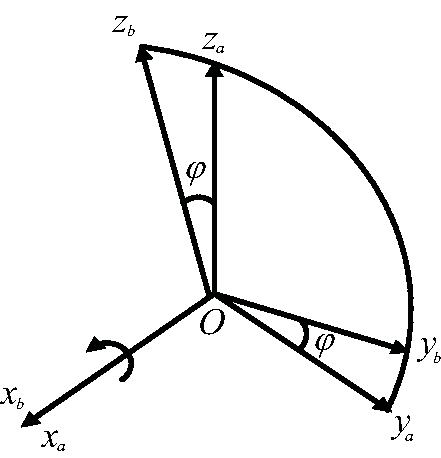
\includegraphics[width=0.77\linewidth]{pic/x}
		\vspace*{-0.5em}
		\caption{绕$x$轴旋转}
		\label{x}
	\end{minipage}
	\begin{minipage}{0.3\linewidth}
		\centering
		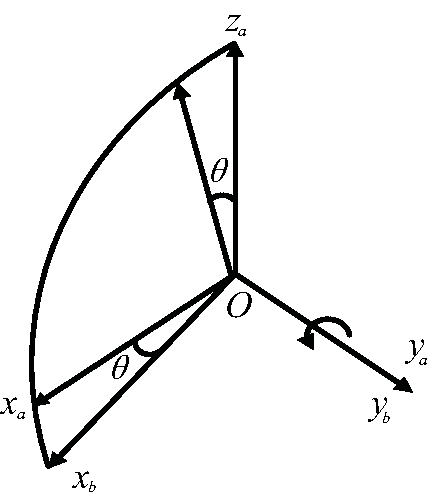
\includegraphics[width=0.78\linewidth]{pic/y}
		\vspace*{-0.5em}
		\caption{绕$y$轴旋转}
		\label{y}
	\end{minipage}
	\begin{minipage}{0.34\linewidth}
		\centering
		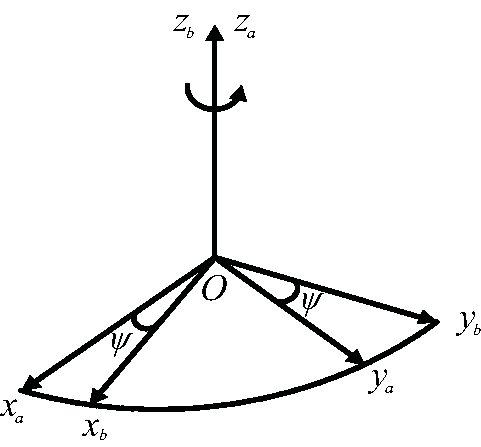
\includegraphics[width=0.85\linewidth]{pic/z}
		\vspace*{-0.5em}
		\caption{绕$z$轴旋转}
		\label{z}
	\end{minipage}
\end{figure}

下面给出两种基元旋转矩阵表示的坐标变换。
\vspace*{0.5em}

\sssection[$ZXZ$旋转顺序]

如图 \ref{ZXZ} 所示,方向余弦矩阵和$ZXZ$顺序欧拉角的关系为
\begin{equation}
	\ubm{C}_{ba} = \ubm{C}_z(\varphi) \ubm{C}_x(\theta) \ubm{C}_z(\psi) = 
	\begin{bmatrix}
		\cos \varphi \cos \psi - \sin \varphi \cos \theta \sin \psi & \cos \varpi \sin \psi + \sin \varphi \cos \theta \cos \psi & \sin \varphi \sin \theta \\
		- \sin \varphi \cos \psi - \cos \varphi \cos \theta \sin \psi & -\sin \varphi \sin \psi + \cos \varphi \cos \theta \cos \psi & \cos \varphi \sin \theta \\
		\sin \theta \sin \psi & -\sin \theta \cos \psi & \cos \theta 
	\end{bmatrix}
\end{equation}
通过与方向余弦矩阵的对应项进行对比,可以计算得到
\begin{equation}
	\begin{cases}
		\, \psi = -\tan^{-1}\left( \dfrac{C_{31}}{C_{32}} \right) \\
		\, \theta = \cos^{-1}\big( C_{33} \big) \\
		\, \varphi = \tan^{-1} \left( \dfrac{C_{13}}{C_{23}} \right)
	\end{cases}
	\label{eq:zxz}
\end{equation}
由公式 \eqref{eq:zxz} 可知,若欧拉角$\theta = 0\degree$,则欧拉转动处于奇异状态,欧拉角$\psi, \varphi$不能唯一确定。因此,$\theta$的取值范围为$0\degree<\theta<180\degree$。
\begin{figure}[!htb]
	\begin{minipage}{0.5\linewidth}
		\centering
		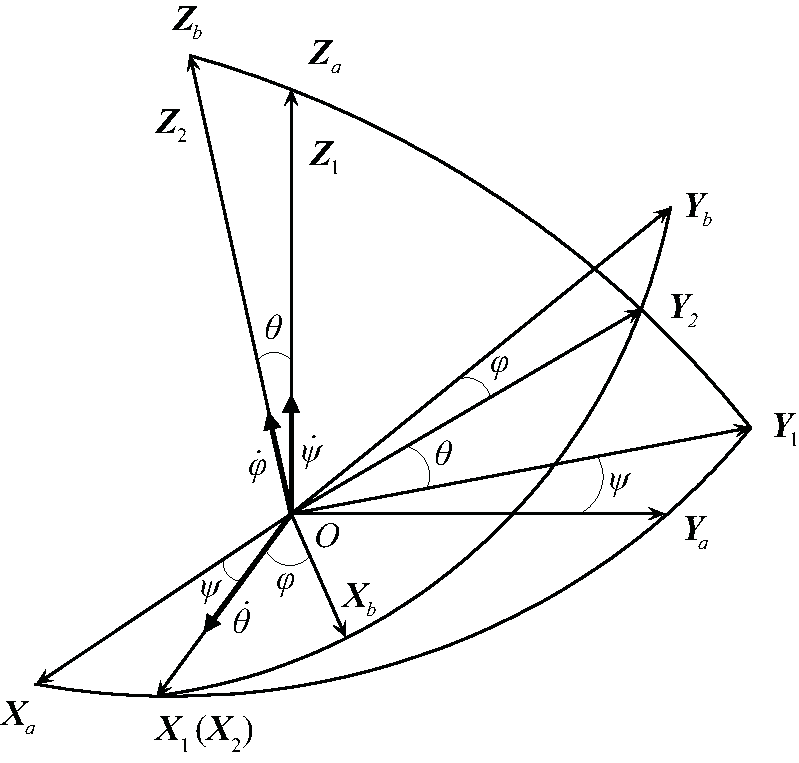
\includegraphics[width=0.8\linewidth]{pic/ZXZ}
		\vspace*{-1em}
		\caption{$ZXZ$顺序欧拉角旋转}
		\label{ZXZ}
	\end{minipage}
	\begin{minipage}{0.5\linewidth}
		\centering
		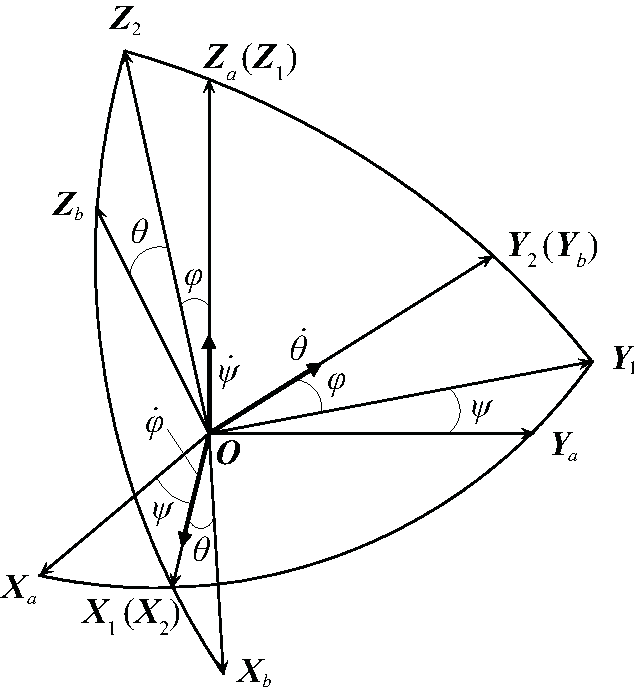
\includegraphics[width=0.695\linewidth]{pic/ZXY}
		\vspace*{-1em}
		\caption{$ZXY$顺序欧拉角旋转}
		\label{ZXY}
	\end{minipage}
\end{figure}


\sssection[$ZXY$旋转顺序]

如图 \ref{ZXY} 所示,方向余弦矩阵和$ZXY$顺序欧拉角的关系
\begin{equation}
	\ubm{C}_{ba} = \ubm{C}_y(\theta)\ubm{C}_x(\varphi)\ubm{C}_z(\psi) =
	\begin{bmatrix}
		\cos \theta \cos \psi - \sin \varphi \sin \theta \sin \psi & \cos \theta \sin \psi + \sin \varphi \sin \theta \cos \psi & -\cos \varphi \sin \theta \\
		-\cos \varphi \sin \psi & \cos \varphi \cos \psi & \sin \varphi \\
		\sin \theta \cos \varphi + \sin \varphi \cos \theta \sin \psi & \sin \theta \sin \psi - \sin \varphi \cos \theta \cos \psi & \cos \varphi \cos \theta 
	\end{bmatrix}
\end{equation}
通过与方向余弦矩阵的对应项进行对比,可以计算得到
\begin{equation}
	\begin{cases}
		\, \psi = -\tan^{-1}\left( \dfrac{C_{21}}{C_{22}} \right) \\
		\, \theta = \sin^{-1}\big( C_{23} \big) \\[0.5em]
		\, \varphi = \tan^{-1} \left( \dfrac{C_{13}}{C_{33}} \right)
	\end{cases}
	\label{eq:zxy}
\end{equation}

由公式 \eqref{eq:zxy} 可知,若欧拉角$\theta = \pm 90 \degree$,则欧拉转动处于奇异状态,欧拉角$\psi, \varphi$在同一平面转动,不能唯一确定。
\vspace*{0.5em}



\subsection{欧拉轴角}
\label{sec: 欧拉轴角}
\vspace*{-1.5em}

\defination[欧拉轴 / 角]
{
	坐标系$S_b$相对坐标系$S_a$的姿态参数可以用单位矢量$\bm{e}$在参考坐标系$S_a$的三个分量$e_x, e_y, e_z$以及绕此转轴的转角$\varPhi$这4个参数来描述,称为\dy[欧拉轴 / 角]{OLZJ}参数。矢量$\bm{e}$称为\dy[欧拉轴]{OLZ},$\varPhi$称为\dy[欧拉转角]{OLZJ}。
}

\sssection[欧拉轴 / 角求方向余项矩阵]

方向余项矩阵$\ubm{C}_{ba}$可由欧拉轴 / 角参数$\bm{e}, \varPhi$得到。
\begin{figure}[!htb]
	\begin{minipage}{0.31\linewidth}
		\centering
		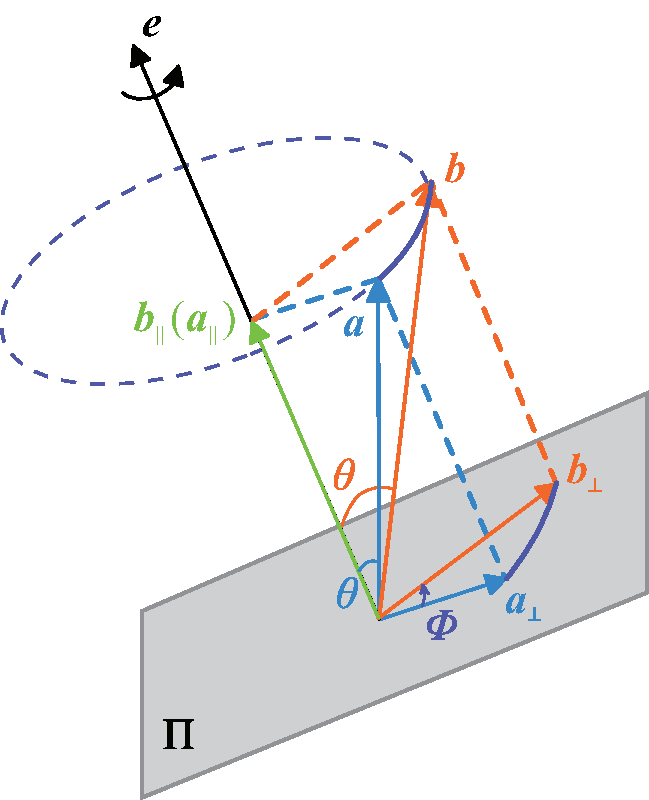
\includegraphics[width=0.9\linewidth]{pic/欧拉轴}
		\vspace*{-1.2em}
		\caption{欧拉轴旋转分解图}
		\label{欧拉轴}
	\end{minipage}
	\begin{minipage}{0.348\linewidth}
		\centering
		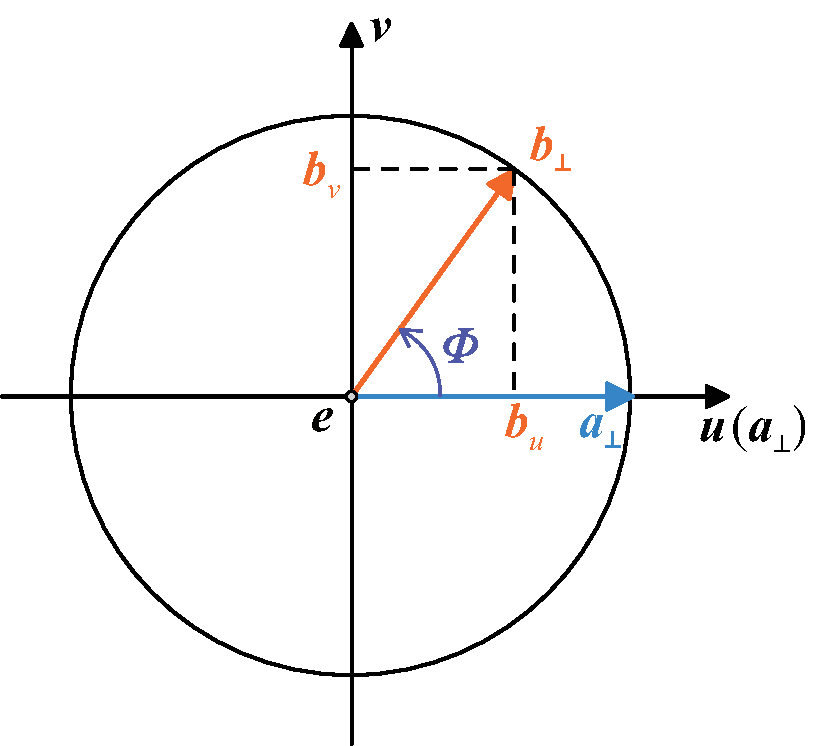
\includegraphics[width=\linewidth]{pic/欧拉轴2}
		\caption{欧拉轴旋转投影图}
		\label{欧拉轴2}
	\end{minipage}
	\begin{minipage}{0.33\linewidth}
		\centering
		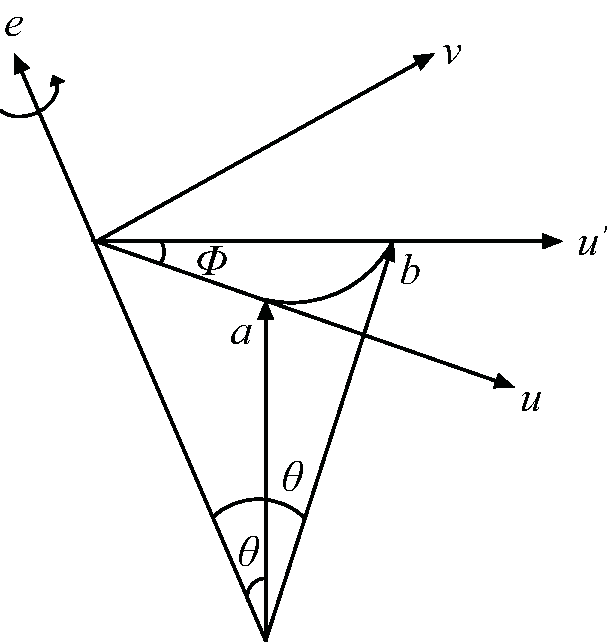
\includegraphics[width=0.913\linewidth]{pic/欧拉轴角}
		\caption{欧拉轴 / 角的坐标变换图}
		\label{欧拉轴角}
	\end{minipage}
\end{figure}

如图 \ref{欧拉轴} 所示,设矢量$\bm{a}$是固定在坐标系$S_a$的任意矢量,矢量$\bm{b}$是固定于坐标系$S_b$中的矢量。将矢量$\bm{a}$绕轴$\bm{e}$旋转一个角度$\varPhi$后得到矢量$\bm{b}$。首先将矢量$\bm{a}$,矢量$\bm{b}$沿轴$\bm{e}$方向和垂直于轴$\bm{e}$方向分解,其平行分量$\bm{a}_{\parallel} = \bm{b}_{\parallel} = \bm{e}$相等,即旋转前后不变,可以发现旋转仅与垂直分量$\bm{a}_{\perp}, \bm{b}_{\perp}$有关。

将垂直分量$\bm{a}_{\perp}, \bm{b}_{\perp}$投影到垂直于轴$\bm{e}$的平面$\Pi$上,如图 \ref{欧拉轴2} 所示。定义单位正交矢量$\bm{u}, \bm{v}$
\begin{align*}
	\bm{u} & = \bm{a}_{\perp} = \dfrac{\bm{e} \times \bm{a}}{\big| \bm{e} \times \bm{a} \big|} = \dfrac{1}{a \sin \theta}(\bm{e} \times \bm{a}) \\
	\bm{v} & = \bm{e} \times \bm{u} = \dfrac{1}{a \sin \theta} \bm{e} \times (\bm{e} \times \bm{a})= \dfrac{1}{a \sin \theta}\big[ \bm{a} - (\bm{e} \cdot \bm{a})\bm{e} \big] 
\end{align*}
将矢量$\bm{b}_{\perp}$分解,得
\begin{equation*}
	\bm{b}_{\perp} = \cos \varPhi \bm{u} + \sin \varPhi \bm{v} = \cos \varPhi \bm{a}_\perp + \sin \varPhi (\bm{a}_\perp \times \bm{e})
\end{equation*}
将矢量$\bm{a}, \bm{b}$用上面的矢量表示为(注:$\bm{a}, \bm{b}$模长相等,即$a=b$)
\begin{align}
	\bm{a} & = a \big( \cos \theta \bm{a}_{\parallel} + \sin \theta \bm{a}_{\perp} \big) 
	= a \big( \cos \theta \bm{e} + \sin \theta \bm{v} \big) \\
	\bm{b} & = b \big( \cos \theta \bm{b}_{\parallel} + \sin \theta \bm{b}_{\perp} \big) 
	= a \big( \cos \theta \bm{e} + \sin \theta \bm{b}_{\perp} \big)
\end{align}
将$\bm{b}_{\perp}$的表达式反代,可以得到
\begin{equation}
	\bm{b} = \cos \varPhi \bm{a} + ( 1 - \cos \varPhi ) (\bm{e} \cdot \bm{a})\bm{e} + \sin \varPhi(\bm{e} \times \bm{a})
\end{equation}
为了写成矩阵形式,我们利用把向量(在坐标系$S_a$的分量)的计算转换为矩阵的形式\footnote[1]{关于$\ubm{e}\ubm{e}^\T$和叉乘矩阵$\ubm{e}^\times$的说明及向量运算矩阵表示的证明,详见 第 \ref{参考内容} 章 \link[参考内容]: \ref{向量运算的矩阵表示} \link[向量运算的矩阵表示]},即
\begin{align*}
	\bm{e} \cdot \bm{a} \cdot \bm{e} = 
	\big[ \bm{i}_a \quad \bm{j}_a \quad \bm{k}_a \big] \,
	\begin{bmatrix}
		e_x \\
		e_y \\
		e_z
	\end{bmatrix}
	\,
	\big[ e_x \quad e_y \quad e_z \big]
	\,
	\begin{bmatrix}
		a_x \\
		a_y \\
		a_z
	\end{bmatrix}
	= \ubm{e}_a^\T \ubm{e} \ubm{e}^\text{T} \ubm{a},
	&& \ubm{e} \times \ubm{a} =
	\big[ \bm{i}_a \quad \bm{j}_a \quad \bm{k}_a \big] \,
	\begin{bmatrix}
		0 & -e_z & e_y \\
		e_z & 0 & -e_x \\
		-e_y & e_x & 0
	\end{bmatrix}
	\,
	\begin{bmatrix}
		a_x \\
		a_y \\
		a_z
	\end{bmatrix}
	= \ubm{e}_a^\T \ubm{e}^\times \ubm{a}
\end{align*}
将$\bm{a}, \bm{b}$在坐标系$S_a$下分解,得
\begin{equation}
	\ubm{e}_a^\T \ubm{b} = \cos \varPhi \ubm{e}_a^\T\ubm{a} + ( 1 - \cos \varPhi ) \ubm{e}_a^\T \ubm{e} \ubm{e}^\text{T} \ubm{a} + \sin \varPhi \ubm{e}_a^\T \ubm{e}^\times \ubm{a}
\end{equation}
两边同时左乘$\big[ \ubm{e}_a^\T \big]^{-1}$,消去$\ubm{e}_a^\T$,可以得到
\begin{align}
	\ubm{b} &= \cos \varPhi \ubm{a} + (1 - \cos \varPhi)\ubm{e}\ubm{e}^\T \bm{a} + \sin \varPhi \ubm{e}_a^\T \ubm{e}^ \times \bm{a} \notag \\
	& = \big[ \cos \varPhi \ubm{E}_3 + (1 - \cos \varPhi) \ubm{e} \ubm{e}^\T + \sin \varPhi \ubm{e}_a^\T \ubm{e}^ \times \big] \ubm{a}
\end{align}
可以得到

\theorem[欧拉轴 / 角参数下的向量旋转矩阵]
{
	在同一坐标系$S_a$下将向量$\bm{a}$绕轴$\bm{e}$旋转$\varPhi$角度得到向量$\bm{b}$,它们的关系为
	\begin{equation}
		\bm{b} = \ubm{R}_{ba} \bm{a}
	\end{equation}
	其中,\dy[向量旋转矩阵]{XLXZJZ}定义为
	\begin{align}
		\ubm{R}_{ba} 
		& = \cos \varPhi \ubm{E}_3 + \big( 1 - \cos \varPhi \big) \ubm{e} \ubm{e}^\T + \sin \varPhi \ubm{e}^{\times} \\
		& = 
		\begin{bmatrix}
			\cos \varPhi + e_x^2 \big( 1 - \cos \varPhi \big) & e_x e_y \big( 1 - \cos \varPhi \big) - e_z \sin \varPhi & e_x e_z \big( 1 - \cos \varPhi \big) + e_y \sin \varPhi \\
			e_x e_y \big( 1 - \cos \varPhi \big) + e_z \sin \varPhi & \cos \varPhi + e_y^2 \big( 1 - \cos \varPhi \big) & e_y e_z \big(1 - \cos \varPhi \big) - e_x \sin \varPhi \\
			e_x e_z \big( 1 - \cos \varPhi \big) - e_y \sin \varPhi & e_y e_z \big( 1- \cos \varPhi \big) + e_x \sin \varPhi & \cos \varPhi + e_z^2 \big( 1- \cos \varPhi \big)
		\end{bmatrix}
		\nomenclature{$\ubm{E}_i$}{$i \times i$的单位矩阵 \nomrefpage}
		\nomenclature{$\ubm{R}_{ba}$}{同一坐标系下向量$\bm{a}$旋转到向量$\bm{b}$的旋转矩阵  \nomrefpage}
	\end{align}
}

而由向量旋转与坐标系旋转的对应关系,可以知道向量旋转矩阵和坐标系旋转矩阵(方向余弦矩阵)互为转置(逆),所以可以得到\footnote[2]{证明详见 第 \ref{参考内容} 章 \link[参考内容]: \ref{向量旋转矩阵和坐标系旋转矩阵的关系} \link[向量旋转矩阵和坐标系旋转矩阵的关系]}

\theorem[欧拉轴 / 角参数下的坐标系旋转矩阵(方向余弦矩阵)]
{
	欧拉轴 / 角参数下的坐标系旋转矩阵(方向余弦矩阵)为
	\begin{align}
		\ubm{C}_{ba} & = (\ubm{R}_{ba})^\T 
		= \big[\cos \varPhi \ubm{E}_3 + \big( 1 - \cos \varPhi \big) \ubm{e} \ubm{e}^\T + \sin \varPhi \ubm{e}^{\times}\big]^\T \notag \\
		& = \cos \varPhi \ubm{E}_3 + \big( 1 - \cos \varPhi \big) (\ubm{e} \ubm{e}^\T)^\T + \sin \varPhi (\ubm{e}^{\times})^\T \notag \\
		& = \cos \varPhi \ubm{E}_3 + \big( 1 - \cos \varPhi \big) \ubm{e} \ubm{e}^\T - \sin \varPhi \ubm{e}^\times \\
		& = 
		\begin{bmatrix}
			\cos \varPhi + e_x^2 \big( 1 - \cos \varPhi \big) & e_x e_y \big( 1 - \cos \varPhi \big) + e_z \sin \varPhi & e_x e_z \big( 1 - \cos \varPhi \big) - e_y \sin \varPhi \\
			e_x e_y \big( 1 - \cos \varPhi \big) - e_z \sin \varPhi & \cos \varPhi + e_y^2 \big( 1 - \cos \varPhi \big) & e_y e_z \big(1 - \cos \varPhi \big) + e_x \sin \varPhi \\
			e_x e_z \big( 1 - \cos \varPhi \big) + e_y \sin \varPhi & e_y e_z \big( 1- \cos \varPhi \big) - e_x \sin \varPhi & \cos \varPhi + e_z^2 \big( 1- \cos \varPhi \big)
		\end{bmatrix}
		\nomenclature{$\ubm{E}_i$}{$i \times i$的单位矩阵 \nomrefpage}
		\nomenclature{$\ubm{R}_{ba}$}{同一坐标系下向量$\bm{a}$旋转到向量$\bm{b}$的旋转矩阵  \nomrefpage}
	\end{align}
}


\sssection[由方向余弦矩阵确定欧拉轴 / 角参数]

若已知方向余弦矩阵$\ubm{C}_{ba}$,可以计算得到欧拉轴 / 角参数,得
\begin{align}
	\cos \varPhi = \dfrac{\text{tr} \ubm{C}_{ba} - 1}{2} \\
	\ubm{e} = \dfrac{1}{2 \sin \varPhi} 
	\begin{bmatrix}
		C_{32} - C_{23} \\
		C_{13} - C_{31} \\
		C_{21} - C_{12}
	\end{bmatrix}
\end{align}
其中,$\text{tr} \ubm{C}_{ba}$是方向余弦矩阵的迹,$\text{tr} \ubm{C}_{ba} = C_{11} + C_{12} + C_{13}$。绕任意轴转动相同的$\varPhi$角,方向余项矩阵的迹不变。

\noindent 将公式展开,对应得到以下3组解:

\noa[1] 当$\text{tr} \ubm{C}_{ba} \neq 3, -1$时,可以直接计算分量$e_x, e_y, e_z$。

\noa[2] 当$\text{tr} \ubm{C}_{ba} = 3$时,此时对应转角$\varPhi = 0, \pm 2 \pi, \pm 4 \pi, \cdots$,方向余弦矩阵$\ubm{C}_{ba}$为单位矩阵,$e_x, e_y, e_z$无法确定。这种情况相当于没有发生转动。

\noa[3] 当$\text{tr} \ubm{C}_{ba} = -1$时,对应转角$\varPhi = \pm \pi, \pm 3 \pi, \pm 5 \pi, \cdots$,此时$\ubm{C}_{ba} = 2 \ubm{e}\ubm{e} - \ubm{E}_3$,则有
\begin{equation}
	\begin{cases}
		\, e_x = \pm \sqrt{\dfrac{1 + C_{11}}{2}}, \qquad e_y = \pm \sqrt{\dfrac{1+ C_{22}}{2}}, \qquad e_z = \pm \sqrt{\dfrac{1 + C_{33}}{2}} \\[0.5em]
		\, e_x e_y = \dfrac{1}{2} C_{12}, \hspace*{3.7em} e_ye_z = \dfrac{1}{2}C_{23}, \hspace*{3.7em} e_ze_x = \dfrac{1}{2} C_{31}
	\end{cases}
\end{equation}
其中,使用后三个方程来判断前三个方程的符号。

\begin{figure}[!htb]
	\centering
	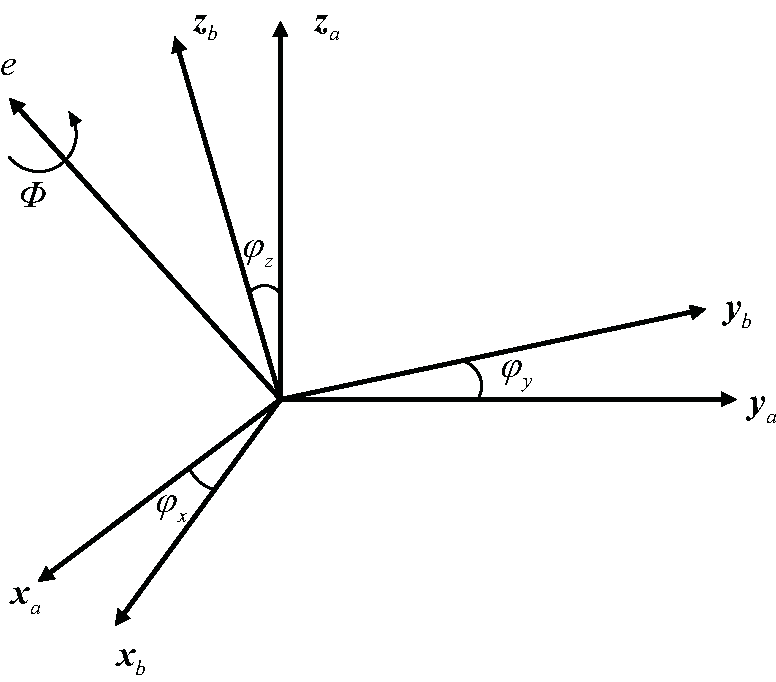
\includegraphics[width=0.42\linewidth]{pic/欧拉轴角变换}
	\vspace*{-1em}
	\caption{欧拉转角与两个坐标系之间的几何关系}
	\label{欧拉转角变换}
\end{figure}


\sssection[欧拉转角的几何意义]

如图 \ref{欧拉转角变换} 所示,令$\varphi_x, \varphi_y, \varphi_z$分别为两个坐标系对应轴之间的夹角,方向余弦矩阵的对焦线上的元素即为这几个角的余弦值,所以
\begin{equation}
	2 \cos \varPhi = \text{tr} \ubm{C}_{ba} - 1 = \cos \varphi_x + \cos \varphi_y + \cos \varphi_z - 1
\end{equation}
利用半角公式$\cos \alpha = 1 - 2 \sin^2 \dfrac{\alpha}{2}$,则
\begin{equation}
	\sin^2 \dfrac{\varPhi}{2} = \dfrac{1}{2} \left( \sin^2 \dfrac{\varphi_x}{2} + \sin^2 \dfrac{\varphi_y}{2} + \sin^2 \dfrac{\varphi_z}{2} \right)
\end{equation}

当偏角较小时,有
\begin{equation}
	\varPhi \approx \dfrac{\sqrt{2}}{2} \sqrt{\varphi_x^2 + \varphi_y^2 + \varphi_z^2}
\end{equation}
这个公式对于评价旋转误差是很有用的。
\vspace*{1em}



\subsection{四元数}
\sssection[四元数的定义{\footnote[1]{四元数章节中的部分内容参考Github上Krasjet的讲义Quaternion\cite{Quaternion}}}]

\defination[四元数]
{
	\dy[四元数]{SYS}的定义和复数类似,唯一的区别就是四元数一共有三个虚部,而复数只有一个。所有的四元数$q \in \mathbb{H}$($\mathbb{H}$代表四元数的发现者 William Rowan Hamilton)都可以写成下面这种形式
	\vspace*{-0.7em}
	\begin{equation}
		q = a + b i + cj +dk \quad (a,b,c,d \in \mathbb{R})
		\nomenclature{$q$}{四元数 \nomrefpage}
		\vspace*{-0.7em}
	\end{equation}
	其中,
	\vspace*{-0.7em}
	\begin{equation}
		i^2 = j^2 = k^2 = i j k = -1
	\end{equation}
}

四元数可以写成向量形式
\begin{equation}
	q = 
	\begin{bmatrix}
		a \\
		b \\
		c \\
		d
	\end{bmatrix}
\end{equation}
同时,通常将四元数的实部与虚部分开,并用一个三维的向量来表示虚部,将它表示为\dy[标量向量有序对]{BLXLYXD}形式
\begin{equation}
	q = \big[ s, \bm{v} \big],
	\quad 
	\bm{v} = 
	\begin{bmatrix}
		x \\
		y \\
		z
	\end{bmatrix} 
	\quad (s,x,y,z \in \mathbb{R})
\end{equation}


\sssection[四元数的模长]
\vspace*{-0.5em}

\defination[四元数的模长]
{
	\dy[四元数的模长]{SYSDMC}(范数)定义为
	\begin{equation}
		\norm[q] = \sqrt{a^2 + b^2 + c^2 + d^2}
		\nomenclature{$\norm[q]$}{四元数的模长(范数)}
	\end{equation}
	用标量向量有序对表示为
	\begin{equation}
		\norm[q] = \sqrt{s^2 + \norm[\bm{v}]^2} = \sqrt{s^2 + \bm{v} \cdot \bm{v}}
	\end{equation}
	\textbf{注:由于四元数是四维向量,其没有明确的物理几何意义。}
}


\sssection[四元数的加减运算]

四元数的加减运算和复数一致,设两个四元数为$q_1 = a + bi + cj + dk,\, q_2 = e + fi +gj + hk$,则
\begin{align}
	q_1 \pm q_2 & = a + bi + cj + dk \pm (e + fi +gj + hk) \notag \\
	& = (a \pm e)  + (b \pm f) i + (c \pm g) j + (d \pm h) k
\end{align}
标量向量对形式的加减与标量和向量的加减运算一致,设两个四元数为$q_1 = \big[s, \bm{v}\big],\, q_2 = \big[ t, \bm{u} \big]$,则
\begin{equation}
	q_1 \pm q_2 = \big[ s \pm t, \bm{v} \pm \bm{u} \big]
\end{equation}


\sssection[四元数的数乘]

一个四元数$q = a +bi +cj +dk$和标量$s$的乘积为
\begin{align}
	sq &= s (a + bi +cj +dk) \notag \\
	& = sa + sbi +scj +sdk
\end{align}
四元数的数乘运算满足交换律,即$sq = qs$.
\vspace*{1em}


\sssection[四元数的乘法]

四元数的乘法和矩阵乘法类似,不遵守交换律,即在一般情况下$q_1 q_2 \neq q_2 q_1$。所以,四元数乘法和矩阵乘法一样有左乘和右乘的区别。即

\noa[1] $q_1 q_2$\quad $q_1\,$\dy[左乘]{ZC}$\,q_2$\quad 或\quad $q_2\,$\dy[右乘]{YC}$\,q_1$.

\noa[2] $q_2 q_1$\quad $q_1\,$\dy[右乘]{YC}$\,q_2$\quad 或\quad $q_2\,$\dy[左乘]{ZC}$\,q_1$.

四元数的乘法满足结合律和分配律。

那么,如果有两个四元数$q_1 = \big[s, \bm{v}\big],\, q_2 = \big[ t, \bm{u} \big]$,则
\begin{align}
	q_1 q_2 & = (a + bi +cj +dk)(e + fi +gj +hk) \notag  \\
	& = ae + afi + agj + ak \notag \\
	& + bei + bfi^2 + bgij + bhik \notag \\
	& + cej + cfji + cgj^2 + chjk \notag \\
	& + dek + dfki + dgkj + dhk^2
\end{align}
利用四元数的性质$i^2 = j^2 = k^2 = i j k = -1$,可以得到
\begin{align}
	 ijk = -1 \, &\xrightarrow{\quad \textstyle \mbox{等式两边同时左乘} \,\, i \quad } \, iijk = -i \hspace*{-8em} &&\Rightarrow \quad jk = i \\
	 ijk = -1 \, &\xrightarrow{\quad \textstyle \mbox{等式两边同时右乘} \,\, k \quad } \, ijkk = -k \hspace*{-8em} &&\Rightarrow \quad ij = k \\
	 jk = i \, &\xrightarrow{\quad \textstyle \mbox{等式两边同时左乘} \,\, j \quad } \, jjk = ji  \hspace*{-8em} &&\Rightarrow \quad ji = -k \\
	 jk = i \, &\xrightarrow{\quad \textstyle \mbox{等式两边同时右乘} \,\, k \quad } \, jkk = ik  \hspace*{-8em} &&\Rightarrow \quad ik = -j \\
	 ij = k \, &\xrightarrow{\quad \textstyle \mbox{等式两边同时左乘} \,\, i \quad } \, iij = ik \hspace*{-8em} &&\Rightarrow \quad ik = -j \\
	 ij = k \, &\xrightarrow{\quad \textstyle \mbox{等式两边同时右乘} \,\, j \quad } \, ijj = kj \hspace*{-8em} &&\Rightarrow \quad kj = -i
\end{align}
将上面的性质整理为表格如表 \ref{四元数基本乘法} 所示。
\begin{table}[!htb]
	\centering
	\setlength{\tabcolsep}{2em}{
	\begin{tabular}{|c|c|c|c|c|}
		\hline
		\rowcolor{Azure2} $\times$ & 1 & $ i $ & $ j $ & $ k $ \\
		\hline
		\cellcolor{Azure2} 1 & 1 & $i$ & $j$ & $k$ \\
		\hline
		\cellcolor{Azure2} $i$ & $i$ & $-1$ &\cellcolor{MistyRose} $k$ & \cellcolor{DarkSlateGray2} $-j$ \\
		\hline
		\cellcolor{Azure2} $j$ & $j$ & \cellcolor{MistyRose} $-k$ & $-1$ & \cellcolor{LightGoldenrod1} $i$ \\
		\hline
		\cellcolor{Azure2} $k$ & $k$ & \cellcolor{DarkSlateGray2} $j$ &  \cellcolor{LightGoldenrod1} $-i$ & $-1$ \\
		\hline
	\end{tabular}
}
\caption{四元数基本向量的乘法计算表(左$\times$上)}
\label{四元数基本乘法}
\end{table}
\vspace*{-2em}

\summarize[
\hspace{1em} 记忆方法:类似于向量的叉乘,将$i,j,k$理解为三维右手坐标系,则$i \times j =k , j \times i = -k$,其余类似。
]

利用表 \ref{四元数基本乘法} ,可以将四元数乘法的结果化简为
\begin{align}
	q_1 q_2 & = ae + afi + agj + ak \notag \\
& + bei + bfi^2 + bgij + bhik \notag \\
& + cej + cfji + cgj^2 + chjk \notag \\
& + dek + dfki + dgkj + dhk^2 \notag \\
& = (a {\color{VioletRed} e} - b {\color{cyan} f} - c{\color{SeaGreen} g} - d{\color{orange} h}) \notag \\
& + (b {\color{VioletRed} e} - a {\color{cyan} f} - d{\color{SeaGreen} g} - c{\color{orange} h}) i \notag \\
& + (c {\color{VioletRed} e} - d {\color{cyan} f} - a{\color{SeaGreen} g} - b{\color{orange} h}) j \notag \\
& + (d {\color{VioletRed} e} - c {\color{cyan} f} - b{\color{SeaGreen} g} - a{\color{orange} h}) k
\end{align}
写成矩阵为
\begin{equation}
		q_1 q_2 = 
		\begin{bmatrix}
			a & -b & -c & -d \\
			b & a & -d & c \\
			c & d & a & -b \\
			d & -c & b & a
		\end{bmatrix}
		\,\, 
		\begin{bmatrix}
		 {\color{VioletRed} e} \\
		 {\color{cyan} f} \\
		 {\color{SeaGreen} g} \\
		 {\color{orange} h} 
		\end{bmatrix}
\end{equation}
同理可得,右乘的结果为
\begin{equation}
	q_2 q_1 = 
	\begin{bmatrix}
		a & -b & -c & -d \\
		b & a & d & c \\
		c & -d & a & b \\
		d & c & -b & a
	\end{bmatrix}
	\,\, 
	\begin{bmatrix}
		{\color{VioletRed} e} \\
		{\color{cyan} f} \\
		{\color{SeaGreen} g} \\
		{\color{orange} h} 
	\end{bmatrix}
\end{equation}
\vspace*{0.5em}


\sssection[Grassmann 积]

为了将四元数的结果写成标量向量有序对,重新整理结果
\begin{align}
	q_1 q_2 & = (ae - ({\color{SeaGreen}bf + cg + dh})) \notag \\
	& + (b {\color{VioletRed} e} + {\color{cyan} a}f +{\color{orange} ch - dg} ) i \notag \\
	& + (c {\color{VioletRed} e} + {\color{cyan} a}g +{\color{orange} df - bh} ) j \notag \\
	& + (d {\color{VioletRed} e} + {\color{cyan} a}h +{\color{orange} bg - cf} ) k \notag 
\end{align}
令
$
\bm{v} = 
\begin{bmatrix}
	b \\
	c \\
	d
\end{bmatrix}
, \,
\bm{u} = 
\begin{bmatrix}
	f \\
	g \\
	h
\end{bmatrix}
$,那么
\begin{align*}
	\bm{v} \cdot \bm{u} &= {\color{SeaGreen}bf + cg + dh} \\
	\bm{v} \times \bm{u} &= 
	\begin{vmatrix}
		\bm{i} & \bm{j} & \bm{k} \\
		b & c & d \\
		f& g & h
	\end{vmatrix}
= ({\color{orange} ch - dg}) \bm{i} + ({\color{orange} df - bh} )\bm{j} + ({\color{orange} bg - cf} )\bm{k}
\end{align*}
所以,$q_1q_2$的结果可以用向量点乘和叉乘的形式表示出来\footnote[1]{其实按照历史的顺序来说,这里第一次提出叉乘的概念。}
\begin{equation}
	q_1 q_2 = \big[ ae - \bm{v} \cdot \bm{u}, a\bm{u} +e \bm{v} + \bm{v} \times \bm{u} \big]
\end{equation}

这个结果称为\dy[Grassmann积]{GRASSMANNJ},一般来说

\theorem[Grassmann 积]
{
	对于任意四元数$q_1= \big[s, \bm{v} \big],\, q_2= \big[ t, \bm{u} \big]$,$q_1q_2$的结果为
	\begin{equation}
		q_1 q_2 = \big[ st - \bm{v} \cdot \bm{u}, s \bm{u} + t \bm{v} + \bm{v} \times \bm{u} \big]
	\end{equation}
}
\vspace*{0.5em}


\sssection[四元数的逆]

因为四元数不遵守交换律,所以类似于矩阵除法,四元数相除等价于乘以它的逆。同样地,也有左除和右除之分,即$pq^{-1}$或$q^{-1}p$,它们的结果一般不同。


\defination[四元数的逆]
{
	如果
	\begin{equation}
		qq^{-1} = q^{-1} q = 1 \quad (q \neq 0)
		\nomenclature{$q^{-1}$}{四元数的逆 \nomrefpage}
	\end{equation}
	那么,我们称$q^{-1}$为四元数$q$的\dy[逆]{N}。
}

直接求解一个四元数的逆$q^{-1}$是非常困难的,但是我们可以使用四元数共轭的性质来求$q^{-1}$。
\vspace*{1em}


\sssection[共轭四元数]
\vspace*{-0.5em}

\defination[共轭四元数]
{
	一个四元数$q = a + bi + cj + dk$的\dy[共轭]{GE}为
	\begin{equation}
		q^* = a - bi - ci -dk
		\nomenclature{$q^*$}{四元数$q$的共轭 \nomrefpage}
	\end{equation}
	如果用标量向量有序对的形式来定义,则$q = \big[ s, \bm{v} \big]$的\dy[共轭]{GE}为
	\begin{equation}
		q^* = \big[ s, -\bm{v} \big]
	\end{equation}
}

共轭四元数的一个非常有用的性质就是
\begin{align}
	q q^* &= \big[s, \bm{v}] \cdot \big[s, - \bm{v}] \notag \\
	& = \big [s^2 - \bm{v} \cdot \bm{v}, s(- \bm{v}) + s \bm{v} + \bm{v} \times (- \bm{v})] \notag \\
	& = \big[s^2 + \bm{v}\cdot \bm{v}, 0] \notag \\
	& = s^2 + x^2 + y^2 + z^2 = \norm[q]^2 \quad \left(\bm{v} = \big[ x, y, z \big]\right) 
\end{align}
因为$(q^*)^* = \big [s, - (- \bm{v})] = \big[s, \bm{v}\big] = q$,则
\begin{equation}
	q^* q = (q^*)(q^*)^* = \norm[q^*]^2 = s^2 + x^2 +y^2 + z^2 = \norm[q]^2 = q q^* 
\end{equation}
这说明,$q^*q = qq^*$。这个特殊的乘法是遵守交换律的。

下面利用四元数的性质求四元数的逆。
\begin{align*}
	q q^{-1} = 1 \, \xrightarrow{\textstyle \quad \mbox{等式两边同时左乘}\, q^* \quad }\, q^* q q^{-1} = 1 &\quad \Rightarrow \quad (q^* q)q^{-1} = q^* \, \xrightarrow{\quad \textstyle q^* q = \norm[q]^2 \quad } \norm[q]^2 \cdot q^{-1} = q^* \notag
\end{align*}
由此可知

\theorem[四元数逆的求解]
{
	四元数的逆可以表示为
	\begin{equation}
		q^{-1} = \dfrac{q^*}{\norm[q]^2}
	\end{equation}
	用这种方法寻找一个四元数的逆会非常高效,我们只需要将一个四元数的共轭除以它的模长的平方就可以得到四元数的逆。特别地对于\dy[单位四元数]{DWSYS}$\norm[q] = 1$来说,它的逆为
	\begin{equation}
		q^{-1} = \dfrac{q^*}{1^2} = q^*
	\end{equation}
}


\sssection[纯四元数]
\vspace*{-0.5em}

\defination[纯四元数]
{
	如果一个四元数实部为0,仅有虚部,即
	\begin{equation}
		v = \big[ 0, \bm{v} \big]
	\end{equation}
	那么我们则称这个四元数$v$为一个\dy[纯四元数]{CXYS}。因为纯四元数仅由虚部的三维向量决定,我们可以将任意的三维向量转换为纯四元数。
}

纯四元数有一个很重要的特性:两个纯四元数$v = \big[ 0, \bm{v} \big], u = \big[ 0, \bm{u} \big]$的乘积为
\begin{align}
	vu &= \big[ 0 - \bm{v} \cdot \bm{u}, 0 + \bm{v} \times \bm{u} \big]  = \big[ - \bm{v} \cdot \bm{u}, \bm{v} \times \bm{u} \big]
	\label{eq: 纯四元数乘法}
\end{align}


\sssection[四元数与三维旋转]

\begin{figure}[!htb]
	\centering
	\begin{minipage}{0.31\linewidth}
		\centering
		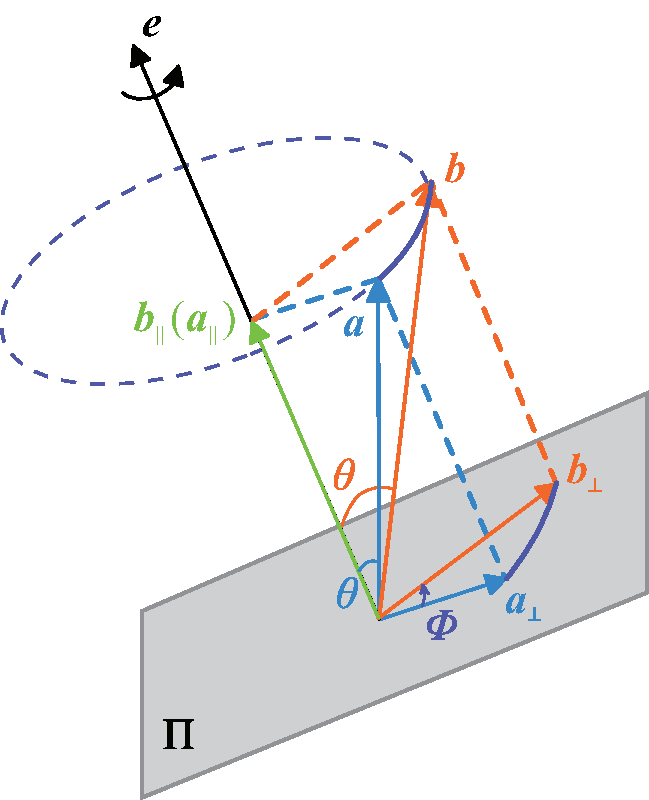
\includegraphics[width=0.9\linewidth]{pic/欧拉轴}
		\vspace*{-1.2em}
		\caption{向量旋转分解图}
		\label{欧拉轴3}
	\end{minipage}\hspace*{7em}
	\begin{minipage}{0.348\linewidth}
		\centering
		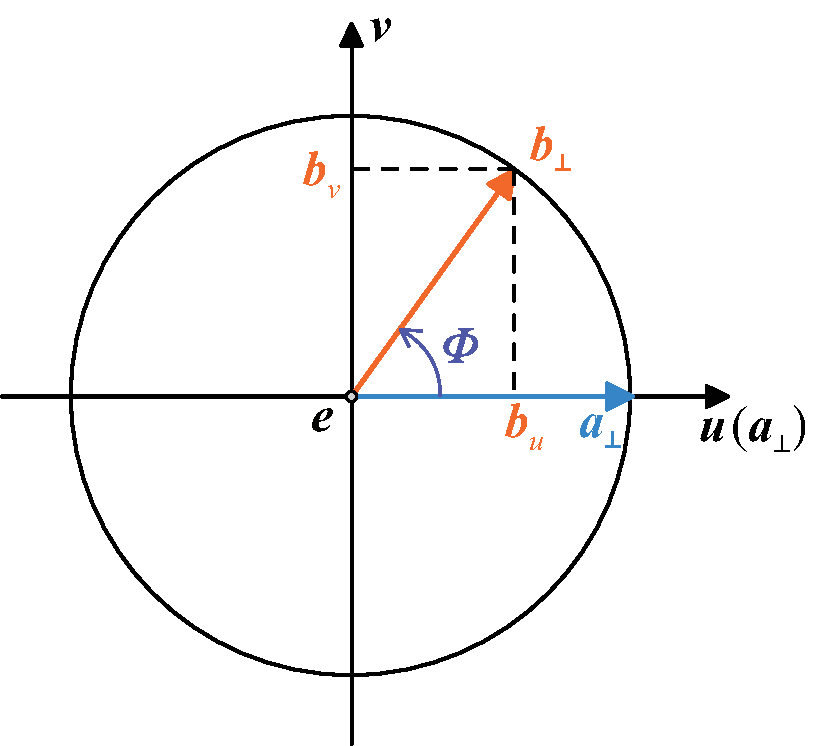
\includegraphics[width=\linewidth]{pic/欧拉轴2}
		\caption{向量旋转投影图}
		\label{欧拉轴4}
	\end{minipage}
\end{figure}

在上个章节 \ref{sec: 欧拉轴角} 中我们知道:如果我们需要将一个向量$\bm{a}$沿着一个用单位向量$\bm{e}$所定义的旋转轴旋转$\varPhi$度,那么我们可以将这个向量$\bm{a}$可以分解为平行于旋转轴的分量$a_{\parallel}$和垂直于旋转轴的分量$a_{\perp}$。旋转后得到的向量$\bm{b}$可以表示为这两个分量分别旋转后之和,即$\bm{b} = \bm{b}_{\parallel} + \bm{b}_{\perp}$。

我们定义这些向量为纯四元数
\begin{align*}
	a &= \big[ 0, \bm{a} \big]  && b = \big[ 0, \bm{b} \big] \\
	a_\perp &= \big[ 0, \bm{a}_\perp \big] && b_\perp = \big[ 0, \bm{b}_\perp \big] \\
	a_\parallel &= \big[ 0, \bm{a}_\parallel \big] && b_\parallel = \big[ 0, \bm{b}_\parallel \big] \\
	e &= \big[0, \bm{e} \big] 
\end{align*}
那么我们可以得到
\begin{equation*}
	a = a_\parallel + a_\perp \qquad \qquad b = b_\parallel + b_\perp
\end{equation*}

如图 \ref{欧拉轴3} 所示,我们知道,旋转前后平行分量$\bm{a}_{\parallel} = \bm{b}_{\parallel} = \bm{e}$相等,即旋转前后不变,下面考虑垂直分量$\bm{a}_{\perp}$的旋转。在上个章节 \ref{sec: 欧拉轴角} 中我们推导过垂直分量$\bm{a}_{\perp}$的旋转公式
\begin{equation*}
	\bm{b}_{\perp} = \cos \varPhi \bm{a}_\perp + \sin \varPhi (\bm{e} \times \bm{a}_\perp )
\end{equation*}

我们可以很容易将$a'_\perp$和$a_\perp$写成四元数的形式,而对于$\bm{a}_\perp \times \bm{e}$,由纯四元数的重要性质,由\eqrefp[eq: 纯四元数乘法]可知,纯四元数$a = \big[ 0, \bm{a_\perp}\big], \, e = \big[ 0, \bm{e} \big]$,那么
\begin{equation*}
	ea_\perp = \big[ - \bm{e} \cdot \bm{a}_\perp, \bm{e} \times \bm{a}_\perp \big]
\end{equation*}
而$\bm{e} \perp \bm{a}_\perp \,\, \Rightarrow \,\, \bm{e} \cdot \bm{a}_\perp = 0$,所以
\begin{align*}
	ea_\perp & = \big[ 0, \bm{e} \times \bm{a}_\perp \big] = \bm{e} \times \bm{a}_\perp
\end{align*}
所以$\bm{a}_{\perp}$旋转公式的四元数表达为
\begin{align}
	b_\perp &= \cos \varPhi a_\perp + \sin \varPhi (ea_\perp) = \big( \cos \varPhi + \sin \varPhi e \big) a_\perp 
\end{align}

令$q = \cos \varPhi + \sin \varPhi e$,则可以得到
\begin{equation}
	b_\perp = q a_\perp
\end{equation}
所以,我们只需要构造一个四元数$q$,就可以完成垂直分量的旋转。对$q$进一步变形,得
\begin{align}
	q &= \cos \varPhi + \sin \varPhi e \notag \\
	& = \big[ \cos \varPhi, \bm{0} \big] + \big[ 0, \sin \varPhi \bm{e} \big] \notag \\
	& = \big[ \cos \varPhi , \sin \varPhi \bm{e} \big] 
\end{align}

如果已经知道旋转轴的坐标
$
\ubm{e} = 
\begin{bmatrix}
	e_x \\
	e_y \\
	e_z
\end{bmatrix}
$
和旋转角$\varPhi$,那么四元数$q$就确定为
\begin{equation}
	q = \big[ \cos \varPhi , \sin \varPhi \bm{e} \big]  = \cos \varPhi + \sin \varPhi e_x \bm{i} + \sin \varPhi e_y \bm{j} + \sin \varPhi e_z \bm{k}
\end{equation}
四元数$q$还有一个性质(注:$\norm[\bm{u}] = 1$)
\begin{align}
	\norm[q] &= \sqrt{\cos^2 \varPhi + (\sin\varPhi \bm{u} \cdot \sin \varPhi \bm{u})} \notag \\
	& = \sqrt{\cos^2 \varPhi + \sin^2 \varPhi(\bm{u} \cdot \bm{u})} \notag \\
	& = \sqrt{\cos^2 \varPhi+ \sin^2 \varPhi} = 1
\end{align}
说明旋转四元数参数$q$是单位四元数,一定意义上表面它所做的变换并不会对原向量进行缩放,是一个纯旋转。
\vspace*{1em}

又因为平行分量旋转前后不改变,即$\bm{b}_\parallel = \bm{a}_\parallel \,\, \Rightarrow \,\,  b_ \parallel = a_ \parallel $所以,向量$\bm{a}$的最终四元数旋转表示为
\begin{align}
	b &= b_\parallel + b_\perp \notag \\
	&= a_\parallel + q a_\perp \qquad \mbox{(其中}\,\, q = \big[ \cos \varPhi, \sin \varPhi \bm{e}\big]\mbox{)}
\end{align}
通过进一步的化简\footnote[1]{由于篇幅所限,此部分化简内容请参见 第 \ref{参考内容} 章 \link[参考内容]: \ref{旋转四元数参数的化简} \link[旋转四元数参数的化简]},可以得到

\theorem[向量旋转的四元数参数]
{
	在同一坐标系下,任意向量$\bm{a}$沿着以单位向量定义的旋转轴$\bm{e}$旋转$\varPhi$度之后的向量$\bm{b}$可以用四元数表达。令$a = \big[ 0, \bm{a} \big], \, q = \left[ \cos \left(\dfrac{1}{2} \varPhi \right), \sin \left(\dfrac{1}{2} \varPhi \right) \bm{e} \right]$,那么
	\begin{equation}
		b = q a q^* = q a q^{-1}
	\end{equation}
	为了更好的理解这个公式的意义,我们可以得到\footnotemark[2]
	\begin{equation}
		b = q a q^* = q q^* a_\parallel + qqa_\perp = a_\parallel + q^2 a_\perp
		\label{旋转四元数的几何意义}
	\end{equation}
	也就是说,$qaq^*$这个变换,实际上可以等价为,对$a$平行于坐标轴的分量$a_\parallel$实施的变换是$qq^*$,这两个变换是互逆的,完全抵消了,也就是没有旋转。而对于正交于旋转轴的分量$a_\perp$,则实施的是两次完全一样的变换$q^2 = qq$,将它旋转$\dfrac{\varPhi}{2} + \dfrac{\varPhi}{2} = \varPhi$度。
}
\footnotetext[2]{公式 \eqref{旋转四元数的几何意义} 是原式公式化简第一步的结果,详情请见\eqrefp[旋转几何意义]。}


由这个公式的由来,可以发现其和上一章节的欧拉轴 / 角的证明是类似的。实际上,旋转四元数参数和欧拉轴 / 角时完全等价的\footnote[3]{其证明见第 \ref{参考内容} 章 \link[参考内容]: \ref{旋转的欧拉轴 / 角参数表达和四元数表达的等价性} \link[旋转的欧拉轴 / 角参数表达和四元数表达的等价性]},即
\begin{equation}
	b = qaq^* = \cos \varPhi \bm{a} + ( 1 - \cos \varPhi ) (\bm{e} \cdot \bm{a})\bm{e} + \sin \varPhi(\bm{e} \times \bm{a})
\end{equation}

若已经知道旋转四元数参数$q=[q_0, \bm{q}]$,则可以很容易获得其对应的旋转角度和旋转轴向量
\begin{align}
	\dfrac{\varPhi}{2} &= \cos^{-1} q_0 \\
	\bm{e} &= \dfrac{\bm{q}}{\sin \big( \cos^{-1} q_0 \big)}
\end{align}


\subsection{欧拉参数}
\sssection[欧拉参数的定义和表示]

为了和方向余弦矩阵具有一致的形式,我们可以将四元数写成矩阵的形式。在四元数的乘法中,我们计算过左乘矩阵和右乘矩阵,若乘数$q = q_0 + q_1i +q_2 j +q_3k$,那么左乘矩阵和右乘矩阵可以分别表示为
\begin{equation}
	L(q) = 
	\begin{bmatrix}
		q_0 & -q_1 & -q_2 & -q_3 \\
		q_1 & q_0 & -q_3 & q_2 \\
		q_2 & q_3 & q_0 & -q_1 \\
		q_3 & -q_2 & q_1 & q_0
	\end{bmatrix},
\,\, \qquad 
	R(q) =
	\begin{bmatrix}
		q_0 & -q_1 & -q_2 & -q_3 \\
		q_1 & q_0 & q_3 & -q_2 \\
		q_2 & -q_3 & q_0 & q_1 \\
		q_3 & q_2 & -q_1 & q_0
	\end{bmatrix}
\end{equation}
同时,对于四元数$q$的共轭$q^*$的乘数矩阵,有
\begin{equation}
	L(q^*) =
	\begin{bmatrix}
		q_0 & q_1 & q_2 & q_3 \\
		-q_1 & q_0 & q_3 & -q_2 \\
		-q_2 & -q_3 & q_0 & q_1 \\
		-q_3 & q_2 & -q_1 & q_0
	\end{bmatrix}
	= [L(q)],
	\,\,\qquad 
	R(q^*) =
	\begin{bmatrix}
		q_0 & q_1 & q_2 & q_3 \\
		-q_1 & q_0 & -q_3 & q_2 \\
		-q_2 & q_3 & q_0 & -q_1 \\
		-q_3 & -q_2 & q_1 & q_0
	\end{bmatrix},
	= [R(q)],
\end{equation}

取
\begin{align*}
	\begin{cases}
		\, q = \big[q_0, \bm{q}\big] = \big[q_0 \quad q_1 \quad q_2 \quad q_3 \big], \\[0.5em]
		\, q_0 = \cos \dfrac{\varPhi}{2}, \qquad q_1 = e_x \sin \dfrac{\varPhi}{2} \\[0.5em]
		\, q_2 = e_y \cos \dfrac{\varPhi}{2}, \qquad q_3 = e_z \sin \dfrac{\varPhi}{2}
	\end{cases}
\end{align*}
其中,四元数$q$是旋转四元数参数,也称为\dy[欧拉参数]{OLCS}。那么我们可以得到
\begin{flalign*}
	b &= q a q^* = L(q)R(q^*)a \, \big[= R(q^*)L(q)a \,\, \big] &\\
	&= 
	\begin{bmatrix}
		q_0 & -q_1 & -q_2 & -q_3 \\
		q_1 & q_0 & -q_3 & q_2 \\
		q_2 & q_3 & q_0 & -q_1 \\
		q_3 & -q_2 & q_1 & q_0
	\end{bmatrix}\,
	\begin{bmatrix}
		q_0 & q_1 & q_2 & q_3 \\
		-q_1 & q_0 & -q_3 & q_2 \\
		-q_2 & q_3 & q_0 & -q_1 \\
		-q_3 & -q_2 & q_1 & q_0
	\end{bmatrix}
	a &\\[0.5em]
	&=
	\begin{bmatrix}
		q_0^2 + q_1^2 + q_2^2 +q_3^2 & q_0q_1 - q_1q_0 -q_2q_3 + q_3q_2 & q_0q_2 + q_1q_3 - q_2q_0 - q_3q_1 & q_0q_3 - q_1q_2 + q_2q_1 - q_3q_0 \\
		q_1q_0 - q_0q_1 + q_3q_2 -q_2q_3 & q_1^2 +q_0^2 - q_3^2 - q_2^2 & q_1q_2 - q_0q_3 - q_3q_0 + q_2q_1 & q_1q_3 + q_0q_2 + q_3q_1 + q_2q_0 \\
		q_2q_0 - q_1q_3 - q_0q_2 + q_1q_3 & q_2q_1 + q_3q_0 + q_0q_3 + q_1q_2 & q_2^2 -q_3^2 + q_0^2 - q_1^2 & q_2q_3 + q_3q_2 - q_0q_1 - q_1q_0 \\
		q_3q_0 + q_2q_1 - q_1q_2 - q_0q_3 & q_3q_1 - q_2q_0 + q_1q_3 - q_0q_2 & q_3q_2 + q_2q_3 +q_1q_0 + q_0q_1 & q_3^2 - q_2^2 - q_1^2 + q_0^2
	\end{bmatrix}
	a &
\end{flalign*}
由于$q_0^2 + q_1^2 + q_2^2 +q_3^2 = 1$(旋转四元数参数$q$是一个单位四元数),所以进一步化简为
\begin{align}
	b &= qaq^* =
	\begin{bmatrix}
		1 & 0 & 0 & 0 \\
		0 & 1 - 2(q_2^2 + q_3^2) & 2(q_1q_2 - q_3q_0) & 2(q_1q_3 + q_2q_0)\\
		0 & 2(q_1q_2 + q_3q_0)  & 1 - 2(q_1^2 + q_3^2) & 2(q_2q_3 - q_1q_0) \\
		0 & 2(q_3q_1 - q_2q_0)& 2(q_2q_3 +q_1q_0) & 1 - 2(q_1^2 + q_2^2)
	\end{bmatrix}
	\,
	\begin{bmatrix}
		a_0 \\
		a_1 \\
		a_2 \\
		a_3
	\end{bmatrix}
\end{align}
其中,$a = \big[a_0 \quad a_1 \quad a_2 \quad a_3 \big]$。由矩阵乘法可知,矩阵的最外圈不会对$a$进行任何变换,而代表$b$的方向仅取决于$\big[a_1 \quad a_2 \quad a_3 \big]$。因此,我们可以删去矩阵最外圈,得到一个$3 \times 3$的矩阵用于三维向量的旋转变换,即

\theorem[欧拉参数表示的向量旋转矩阵]
{
	在同一坐标系下,任意向量$\bm{a}$沿着以单位向量定义的旋转轴$\bm{e}$旋转$\varPhi$角度之后的向量$\bm{b}$可以用矩阵乘法来获得
	\begin{equation}
		\begin{cases}
			\, q_0 = \cos \dfrac{\varPhi}{2}\\[0.5em]
			\, q_1 = e_x \sin \dfrac{\varPhi}{2} \\[0.5em]
			\, q_2 = e_y \sin \dfrac{\varPhi}{2}\\[0.5em]
			\, q_3 = e_z \sin \dfrac{\varPhi}{2}
		\end{cases}
		\,\, \Longrightarrow \,\,
		\ubm{b} = 
		\ubm{R}_{ba}(\ubm{q})
	\ubm{a},
	\,\,
	\ubm{R}_{ba}(\ubm{q}) = 
	\begin{bmatrix}
		1 - 2(q_2^2 + q_3^2) & 2(q_1q_2 - q_3q_0) & 2(q_1q_3 + q_2q_0)\\
		2(q_1q_2 + q_3q_0)  & 1 - 2(q_1^2 + q_3^2) & 2(q_2q_3 - q_1q_0) \\
		2(q_3q_1 - q_2q_0)& 2(q_2q_3 +q_1q_0) & 1 - 2(q_1^2 + q_2^2)
	\end{bmatrix}
	\end{equation}
}

同样地,由向量旋转与坐标系旋转的对应关系,可以知道向量旋转矩阵和坐标系旋转矩阵(方向余弦矩阵)互为转置(逆),所以可以得到\footnote[1]{证明详见 第 \ref{参考内容} 章 \link[参考内容]: \ref{向量旋转矩阵和坐标系旋转矩阵的关系} \link[向量旋转矩阵和坐标系旋转矩阵的关系]}

\theorem[欧拉参数表示的坐标旋转矩阵(方向余弦矩阵)]
{
	欧拉参数表示的坐标旋转矩阵(方向余弦矩阵)为
	\begin{equation}
		\begin{cases}
			\, q_0 = \cos \dfrac{\varPhi}{2}\\[0.5em]
			\, q_1 = e_x \sin \dfrac{\varPhi}{2} \\[0.5em]
			\, q_2 = e_y \sin \dfrac{\varPhi}{2}\\[0.5em]
			\, q_3 = e_z \sin \dfrac{\varPhi}{2}
		\end{cases}
		\,\, \Longrightarrow \,\,
		\ubm{b} = 
		\ubm{C}_{ba}(\ubm{q})
		\ubm{a},
		\,\,
		\ubm{C}_{ba}(\ubm{q}) = 
		\begin{bmatrix}
			1 - 2(q_2^2 + q_3^2) & 2(q_1q_2 + q_3q_0) & 2(q_1q_3 - q_2q_0)\\
			2(q_1q_2 - q_3q_0)  & 1 - 2(q_1^2 + q_3^2) & 2(q_2q_3 + q_1q_0) \\
			2(q_3q_1 + q_2q_0)& 2(q_2q_3 - q_1q_0) & 1 - 2(q_1^2 + q_2^2)
		\end{bmatrix}
	\end{equation}
}

虽然三维旋转的矩阵形式(欧拉参数)可能不如四元数的形式简单,而且占用更多的空间,但是对于大批量的转换,使用\textbf{预先计算}好的矩阵是比四元数乘法更有效率的。


我们知道方向余弦矩阵的欧拉轴 / 角参数表述为
\begin{equation}
	\ubm{C}_{ba} = \cos \varPhi \ubm{E}_3 +(1 - \cos \varPhi)\ubm{e}\ubm{e} - \sin \varPhi \ubm{e}^\times
\end{equation}
类似的,我们也可以将欧拉参数写成矩阵运算的形式,注意到
\begin{align*}
	q_0 &= \cos \dfrac{\varPhi}{2}\\[0.5em]
	\ubm{q} &= \ubm{e} \sin \dfrac{\varPhi}{2} \\[0.5em]
	\ubm{q} &= \ubm{e} \sin \dfrac{\varPhi}{2} \\[0.5em]
	\ubm{q}^{\times} &= 
	\begin{bmatrix}
		0 & -e_z\sin \dfrac{\varPhi}{2} & e_y\sin \dfrac{\varPhi}{2} \\[0.8em]
		e_z\sin \dfrac{\varPhi}{2} & 0 & -e_x\sin \dfrac{\varPhi}{2} \\[0.8em]
		-e_y\sin \dfrac{\varPhi}{2} & e_x\sin \dfrac{\varPhi}{2} & 0
	\end{bmatrix}
	= \ubm{e}^\times \sin \dfrac{\varPhi}{2}
\end{align*}
\begin{align*}
	\ubm{q}^T \ubm{q} &= 
	\bigg[ e_x \sin \dfrac{\varPhi}{2} \quad e_y \sin \dfrac{\varPhi}{2} \quad e_z \sin  \dfrac{\varPhi}{2} \bigg]
	\,
	\begin{bmatrix}
		e_x \sin \dfrac{\varPhi}{2} \\[0.8em]
		 e_y \sin \dfrac{\varPhi}{2} \\[0.8em]
		 e_z \sin  \dfrac{\varPhi}{2}
	\end{bmatrix}
	= (e_x^2 +e_y^2 + e_z^2)\sin^2 \dfrac{\varPhi}{2} = \sin^2 \dfrac{\varPhi}{2}
\end{align*}
对欧拉轴 / 角参数型方向余弦矩阵进行变换,得
\begin{align}
	\ubm{C}_{ba} &= \cos \varPhi \ubm{E}_3 + (1 - \cos \varPhi)\bm{e}\ubm{e} - \sin \varPhi \ubm{e}^\times \notag \\
	&= \left( 1 - 2\sin^2 \dfrac{\varPhi}{2} \right) \ubm{E}_3 + 2 \sin^2 \dfrac{\varPhi}{2} \ubm{e}\ubm{e} - 2 \sin \dfrac{\varPhi}{2} \cos \dfrac{\varPhi}{2} \ubm{e}^\times \notag \\[0.5em]
	&= \left( 1 - 2\sin^2 \dfrac{\varPhi}{2}\right) \ubm{E}_3 + 2\left( \ubm{e} \sin \dfrac{\varPhi}{2}\right)\left( \ubm{e} \sin \dfrac{\varPhi}{2}\right) - 2 \cos \dfrac{\varPhi}{2} \left( \ubm{e}^\times \sin \dfrac{\varPhi}{2} \right) \notag \\
	& = \big( 1 - 2\ubm{q}^\T \ubm{q} \big) \ubm{E}_3 + 2 \ubm{q}\ubm{q}^\T - 2 q_0 \ubm{q}^\times 
\end{align}


\sssection[欧拉参数与方向余弦矩阵之间的转换]

通过比对欧拉参数矩阵和方向余弦矩阵系数
\begin{equation}
	\ubm{C}_{ba} = 
	\begin{bmatrix}
		C_{11} & C_{12} & C_{13} \\
		C_{21} & C_{22} & C_{23} \\
		C_{31} & C_{32} & C_{33}
	\end{bmatrix}
	= 
	\begin{bmatrix}
		1 - 2(q_2^2 + q_3^2) & 2(q_1q_2 + q_3q_0) & 2(q_1q_3 - q_2q_0)\\
		2(q_1q_2 - q_3q_0)  & 1 - 2(q_1^2 + q_3^2) & 2(q_2q_3 + q_1q_0) \\
		2(q_3q_1 + q_2q_0)& 2(q_2q_3 - q_1q_0) & 1 - 2(q_1^2 + q_2^2)
	\end{bmatrix}
\end{equation}
当方向余弦矩阵系数已知时,可以求出四元数$q$
\begin{equation}
	\begin{cases}
		\, q_0 =  \pm \dfrac{1}{2} \sqrt{1 + C_{11} + C_{22} + C_{33}} \\[0.8em]
		\, q_1 = \dfrac{1}{4q_0}(C_{23} - C_{32}) \\[0.8em]
		\, q_2 = \dfrac{1}{4q_0}(C_{31} - C_{13}) \\[0.8em]
		\, q_3 = \dfrac{1}{4q_0}(C_{12} - C_{21})
	\end{cases}
	\label{eq: q_0}
\end{equation}

当$q_0 = 0$时,公式 \eqref{eq: q_0} 是奇异的,无法求解$q_1, q_2, q_3$,通过比对系数还可以获得其余三组解:

\begin{equation}
	\begin{cases}
		\, q_1 = \pm \dfrac{1}{2} \sqrt{1 + C_{11} - C_{22} - C_{33}} \\[0.8em]
		\, q_2 = \dfrac{1}{4q_1}(C_{12} + C_{21}) \\[0.8em]
		\, q_3 = \dfrac{1}{4q_1}(C_{13} + C_{31}) \\[0.8em]
		\, q_0 = \dfrac{1}{4q_1}(C_{23} - C_{32})
	\end{cases}
\end{equation}

\begin{equation}
	\begin{cases}
		\, q_2 = \pm \dfrac{1}{2} \sqrt{1 - C_{11} + C_{22} - C_{33}} \\[0.8em]
		\, q_3 = \dfrac{1}{4q_2}(C_{23} + C_{32}) \\[0.8em]
		\, q_0 = \dfrac{1}{4q_2}(C_{31} - C_{13}) \\[0.8em]
		\, q_1 = \dfrac{1}{4q_2}(C_{12} + C_{21})
	\end{cases}
\end{equation}
\clearpage
\vspace*{-3em}
\begin{equation}
	\begin{cases}
		\, q_3 = \pm \dfrac{1}{2} \sqrt{1 - C_{11} - C_{22} + C_{33}} \\[0.8em]
		\, q_0 = \dfrac{1}{4q_3}(C_{12} - C_{21}) \\[0.8em]
		\, q_1 = \dfrac{1}{4q_3}(C_{13} + C_{31}) \\[0.8em]
		\, q_2 = \dfrac{1}{4q_3}(C_{23} + C_{32})
	\end{cases}
\end{equation}

所以,一共有四种计算方法求解欧拉参数$q = \big[ q_0 \quad q_1 \quad q_2 \quad q_3 \big]$,为了降低计算结果的误差,我们选取奇异性最小的一组解,即通过计算
\begin{equation}
	\begin{cases}
		\, q_0 =  \pm \dfrac{1}{2} \sqrt{1 + C_{11} + C_{22} + C_{33}} \\[0.8em]
		\, q_1 = \pm \dfrac{1}{2} \sqrt{1 + C_{11} - C_{22} - C_{33}} \\[0.8em]
		\, q_2 = \pm \dfrac{1}{2} \sqrt{1 - C_{11} + C_{22} - C_{33}} \\[0.8em]
		\, q_3 = \pm \dfrac{1}{2} \sqrt{1 - C_{11} - C_{22} + C_{33}}
	\end{cases}
\quad 
\xrightarrow{\quad \textstyle \mbox{选取最大的一个作为解} \quad } \quad 
	q_j = \max_{i = 1,2,3,4} q_i
\end{equation}
这样以后,后面计算用到的$\dfrac{1}{4q_j}$的奇异性最小,计算的精度最高。
\vspace*{0.5em}

上面计算得到的欧拉参数称为从坐标系$S_a$到坐标系$S_b$的欧拉参数,或者坐标系$S_b$相对于坐标系$S_a$的欧拉参数。为了更明确的显示坐标系的转换关系,将其记为$q_{ba}$。
\vspace*{1em}


\sssection[相继转动的欧拉参数表示]

假设有两个表示沿着不同轴,不同角度旋转的非零四元数$q_{ba}, q_{cb}$,我们先对$a$进行$q_{ba}$变换得到$b$
\begin{equation*}
	b = q_{ba} a q_{ba}^*
\end{equation*}
再对$b$进行$q_{cb}$变换得到$c$
\begin{align*}
	c &= q_{cb} b q_{cb}^* \\
	&= q_{cb}q_{ba} a q_{ba}^* q_{cb}^*
\end{align*}
下面给出一个引理

\lemma[]
{
	对任意四元数$q_1 = \big[ s, \bm{v} \big],\, q_2 = \big[t, \bm{u} \big]$,有
	\vspace*{-0.5em}
	\begin{equation}
		q_1^* q_2^* = (q_2q_1)^*
	\end{equation}
}
\label{lemma:1-1}
\proof 由Grassmann积,
\begin{flalign*}
	\text{LHS} &= q_1^*q_2^* \\
	&= \big[ s, -\bm{v} \big] \cdot \big[ t, -\bm{u} \big] \\
	&= \big[ st - (-\bm{v}) \cdot (-\bm{u}), s (-\bm{u}) + t (-\bm{v}) + (-\bm{v}) \times (-\bm{u}) \big] \\
	&= \big[ st - \bm{v} \cdot \bm{u}, -s\bm{u}- t \bm{v} + \bm{v} \times \bm{u} \big] 
\end{flalign*}
\begin{flalign*}
	\text{RHS} &= (q_2q_1)^* \\
	&= \left( \big[ t, \bm{u} \big] \cdot \big[ s, \bm{v} \big] \right)^* \\
	&= \big[ ts - \bm{u} \cdot \bm{v}, t \bm{v} + s \bm{u} + \bm{u} \times \bm{v} \big]^* \\
	&= \big[st - \bm{v} \cdot \bm{u}, -s \bm{u} - t \bm{v} - \bm{u} \times \bm{v} \big] \\
	&= \big[ st - \bm{v} \cdot \bm{u}, -s\bm{u}- t \bm{v} + \bm{v} \times \bm{u} \big] = \text{LHS} 
\end{flalign*}
\hfill $\square$

所以,根据\ref{lemma:1-1} 可以得到
\begin{align}
	c &= q_{cb}q_{ba} a q_{ba}^* q_{cb}^* \notag \\
	&= (q_{cb} q_{ba}) a (q_{cb}q_{ba})^* \notag \\
	& = q_{ca} a q_{ca}^*
\end{align}
其中,$q_{ca} = q_{cb} \cdot q_{ba}$。也就是说,坐标系$S_a$通过两次旋转$q_{ba}, q_{cb}$后得到坐标系$S_c$等价于一次旋转$q_{ca}$。

\warn
[
\textbf{\large 旋转顺序与四元数乘法顺序}\\
\hspace*{1.8em} 我们先进行的是$q_{ba}$变换,再进行$q_{cb}$变换,其对应的四元数乘法为$q_{ca} = q_{cb} \cdot q_{ba}$,即先进行的变换放在后面,对于多旋转来说也符合这个计算顺序。
]

我们这个只是两个旋转的复合,很容易可以推广到多旋转,即
\begin{equation}
	d = q_{dc}(q_{cb} q_{ba}) a (q_{cb} q_{ba})^*q_3^* = (q_{dc} q_{cb} q_{ba}) a (q_{dc} q_{cb} q_{ba})^* = q_{da} a q_{da}^*
\end{equation}


\subsection{其他类型的姿态参数}

\sssection[罗德里格(Rodrigues)参数]

\dy[罗德里格参数]{LDLGCS}是三个标量,也是从欧拉轴 / 角参数演化过来的,其定义是
\begin{equation}
	\ubm{\rho} \triangleq \ubm{e} \tan \dfrac{\varPhi}{2} = \dfrac{1}{q_0} \ubm{q}
\end{equation}

罗德里格参数与欧拉参数相比,其优点是参数少;缺点是在某些时候(如$\varPhi$接近$\pm \pi$时),参数会接近无限大,而欧拉参数的绝对值不会超过1。

罗德里格参数的方向余弦矩阵表示为
\begin{align}
	\ubm{C}_{ba} &= 
	\dfrac{(1 - \ubm{\rho}\ubm{\rho})\ubm{E}_3 + 2 \ubm{\rho} \ubm{\rho} - 2 \ubm{\rho}^\times}{1 + \ubm{\rho}\ubm{\rho} } \\[0.5em]
	&=
	\dfrac{1}{1 + \rho_1^2 + \rho_2^2 + \rho_3^2 }
	\begin{bmatrix}
		1 + \rho_1^2 - \rho_2^2 - \rho_3^2 & 2(\rho_1\rho_3 - \rho_3) & 2(\rho_!\rho_3 - \rho_2) \\
		2(\rho_2 \rho_1 - \rho_3) & 1 - \rho_1^2 + \rho_2^2 - \rho_3^2 &2(\rho_2 \rho_3 + \rho_1) \\
		2(\rho_3 \rho)1 + \rho_2) & 2(\rho_3\rho_2 - \rho_1) & 1 - \rho_1^2 - \rho_2^2 + \rho_3^2
	\end{bmatrix}
\end{align}
\vspace*{0.5em}


\sssection[修正的罗德里格参数]

基于罗德里格参数在$\varPhi$接近$\pm \pi$时,参数会接近无限大的缺点,又提出了一种\dy[修正的罗德里格参数]{XZDLDLGCS},其定义为
\begin{equation}
	\ubm{\rho}^* \triangleq \ubm{e} \tan \dfrac{\varPhi}{4} = \dfrac{\sin (\varPhi / 2)}{1 + \cos (\varPhi / 2)} \ubm{e} = \dfrac{1}{1 + q_0} \ubm{q}
\end{equation}

根据定义可知,修正的罗德里格参数只有在欧拉转角为$\pm 2 \pi$时才会变为奇异点,而实际应用中航天器相对参考坐标系的欧拉转角不需要表示到$\pm 2 \pi$,这经常在工程中使用。




\section{姿态运动学方程}

研究\textbf{姿态参数的变化与角速度矢量$\bm{\omega}_{ba}$的关系}的学科称为\dy[姿态运动学]{ZTYDX}。实际上,$\omega_{ba}$的方向就是欧拉轴 / 角姿态参数中的瞬时旋转轴$\bm{e}$的方向,$\bm{\omega_{ba}}$的数值大小即为$\d \varPhi / \d t$。

角速度$\bm{\omega}_{ba}$的表示方法有两种:

\noa[1] $\bm{\omega}_{ba}$在参考坐标系$\bm{S}_a$中的分量矩阵$\omega_{ba}^a$.

\noa[2] $\bm{\omega}_{ba}$在参考坐标系$\bm{S}_b$中的分量矩阵$\omega_{ba}^b$.
\vspace*{0.5em}

\subsection{向量的时间导数}
设坐标系$S_a$以角速度
\begin{equation}
	\bm{\omega}_a = \bm{\omega}_{xa} \bm{i}_a + \bm{\omega}_{ya} \bm{j}_a + \bm{\omega}_{za} \bm{k}_a 
\end{equation}
相对惯性空间旋转,$\bm{u}$为一个变化的向量
\begin{equation*}
	\bm{u} = \bm{u}_{xa} \bm{i}_a + \bm{u}_{ya} \bm{j}_a + \bm{u}_{za} \bm{k}_a
\end{equation*}
则矢量$\bm{u}$在惯性空间对时间$t$的导数为
\begin{equation}
	\dfrac{\d \bm{u}}{\d t} = \left( \dfrac{\d \bm{u}_{xa}}{\d t}\bm{i}_a + \dfrac{\d \bm{u}_{ya}}{\d t} \bm{j}_a + \dfrac{\d \bm{u}_{za}}{\d t} \bm{k}_a \right) + \left(\bm{u}_{xa} \dfrac{\d \bm{i}_a}{\d t} + \bm{u}_{ya} \dfrac{\d \bm{j}_A}{\d t} + \bm{u}_{za} \dfrac{\d \bm{k}_a}{\d t}\right)
\end{equation}
\vspace*{0.1em}

\noindent
\begin{minipage}{0.6\linewidth}
	其中,等号右侧前3项表示在坐标系$S_a$下每一分量对时间的导数, 再求向量和,它表示向量$\bm{u}$相对于向量基$\bm{e}_a$的时间变化率,可以\\[0.2em]
	写为$\dfrac{\delta \bm{u}}{\delta t}$ \nomenclature{$\dfrac{\delta  \bm{u}}{\delta t}$}{向量$\bm{u}$相对于运动向量基$\bm{e}_a$的时间变化率,相对导数 \nomrefpage},表示\dy[相对导数]{XDDS},以便与\dy[绝对导数]{JDDS}$\dfrac{\d \bm{u}}{\d t}$ \nomenclature{$\dfrac{\d \bm{u}}{\d t}$}{向量$\bm{u}$相对于惯性向量基的时间变化率,绝对导数 \nomrefpage}区分。等号右侧后三\\[0.2em]
	项都是单位基向量对时间的导数,如图 \ref{基向量的转动} 所示。
	
	\qquad 设$\bm{e}$是固定在坐标系$S_a$中的单位基向量,$\bm{\omega}$是基向量转动的角速度。在$t = t_0$时刻,$\bm{e}$的末端位于$a$点,经过$\Delta t$时间后,$\bm{e}$转动到$\bm{e}'$,其末端相应的转动到$a'$点。记$aa'$的圆心为点$O$,$\bm{e}$与$\bm{\omega}$之间的夹角为$\theta$,则由图 \ref{基向量的转动} 可知$\angle aOa' = \bm{\omega} \Delta t,\, \, aa' = \bm{\omega}\Delta t |\bm{e}| \sin \theta$。当$\Delta t$趋近于0时,弧$\wideparen{aa'}$逼近弦长$aa'$,其方向趋近于圆在$a$点的切线$\bm{\tau}$。所以,$\Delta \to 0 \Rightarrow \wideparen{aa'} = aa' = \bm{\omega} \times \bm{e}\Delta t$。由向量导数的定义,有
	\begin{equation}
		\dfrac{\d \bm{e}}{\d t} = \lim\limits_{\Delta \to 0}\dfrac{\wideparen{aa'}}{\Delta t} = \lim\limits_{\Delta t \to 0} \dfrac{\bm{\omega} \times \bm{e} \Delta t}{\Delta t} = \bm{\omega} \times \bm{e}
	\end{equation}
\end{minipage}
\begin{minipage}{0.4\linewidth}
	\centering
	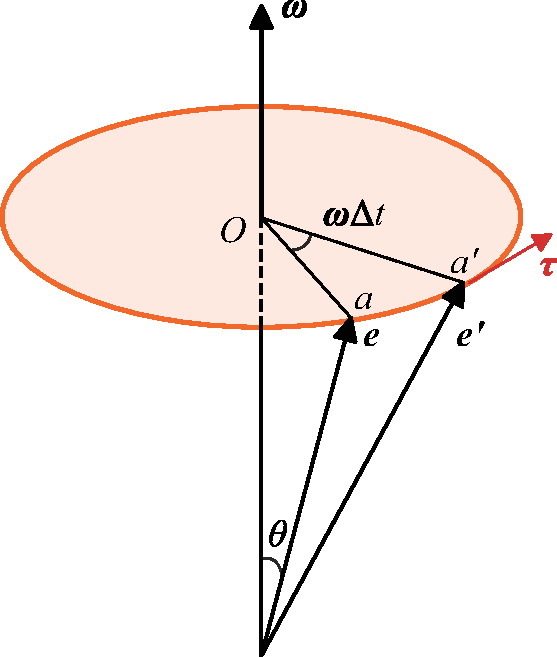
\includegraphics[width=0.8\linewidth]{pic/向量转动}
	\captionof{figure}{基向量的转动}
	\label{基向量的转动}
\end{minipage}
\vspace*{0.5em}

\noindent 展开可得
\vspace*{0.5em}
\begin{equation}
	\dfrac{\d \bm{u}}{\d t} = \left( \dfrac{\d \bm{u}_{xa}}{\d t}\bm{i}_a + \dfrac{\d \bm{u}_{ya}}{\d t} \bm{j}_a + \dfrac{\d \bm{u}_{za}}{\d t} \bm{k}_a \right) + \bm{\omega}_a \times (\bm{u}_{xa} \bm{i}_a + \bm{u}_{xa}\bm{i}_a + \bm{u}_{ya}\bm{j}_a + \bm{u}_{za}\bm{k}_a)
\end{equation}

\noindent 即
\vspace*{0.5em}
\begin{equation}
	\dfrac{\d \bm{u}}{\d t} = \dfrac{\delta \bm{u}}{\d t} + \bm{\omega}_a \times \bm{u}
\end{equation}

\newpage



\subsection{方向余弦矩阵的微分方程}
\sssection[方向余项矩阵的微分方程]

\noindent 由
\begin{equation*}
	\ubm{e}_a = \ubm{C}_{ab}\ubm{e}_b \, \xrightarrow{\quad \textstyle \mbox{两边取转置} \quad} \,  \ubm{e}_a^\T = \big( \ubm{C}_{ab} \ubm{e}_b \big)^\T  \quad \Rightarrow \quad \ubm{e}_a^\T = \ubm{e}_b^\T \ubm{C}_{ab}^\T = \bm{e}_b^\T \ubm{C}_{ba}
\end{equation*}
用$\dot{\,}$表示向量在坐标系$S_a$中的时间导数,则有$\dfrac{\d \bm{e}_a}{\d t} = \dot{\ubm{e}}_a = 0$,且根据向量的时间导数,可以得到
\begin{equation}
	\dot{\ubm{e}}_b^\T = \bm{\omega}_{ba} \times \ubm{e}_b^\T
\end{equation}
对角速度$\bm{\omega}_{ba}$在$S_b$坐标系下的分解,并由广义向量叉乘运算\footnote[1]{关于广义向量叉乘运算的定义,详见 第 \ref{参考内容} 章 \link[参考内容]:\ref{广义向量叉乘运算}  \link[广义向量叉乘运算]},可得
\begin{equation}
	\dot{\ubm{e}}_b^\T = \bm{\omega}_{ba}^\T \ubm{e}_b \times \ubm{e}_b^\T = \ubm{e}_b^\T \ubm{\omega}_{ba}^\times 
\end{equation}
在坐标系$\bm{S}_a$中对两边求导,
\begin{flalign*}
	\ubm{0}^\T &= \dot{\ubm{e}}_b^\T \ubm{C}_{ba} + \bm{e}_b^\T \dot{\ubm{C}}_{ba} \\
	&= \ubm{e}_b^\T \ubm{\omega}_{ba}^\times \ubm{C}_{ba} + \ubm{e}_b^\T \dot{\ubm{C}}_{ba} \\
	& = \ubm{e}_b^\T \big( \ubm{\omega}_{ba}^\times \ubm{C}_{ba} + \dot{\ubm{C}}_{ba} \big) 
\end{flalign*}
于是可以得到

\theorem[方向余弦矩阵的微分方程]
{
	方向余弦矩阵$\bm{C}_{ba}$的微分方程为
	\begin{equation}
		\dot{\ubm{C}}_{ba} = - \ubm{C}_{ba} \ubm{\omega}_{ba}^\times
	\end{equation}
	\textbf{\color{red} 注意:$\ubm{\omega}_{ba}$是$\bm{\omega}_{ba}$在坐标系$S_b$下的分量。}
}


也就是说,如果已知$\bm{\omega}(t)$,可以通过积分法求得方向余弦矩阵$\ubm{C}_{ba}(t)$的时间表达式。可以利用
\begin{equation*}
	\ubm{C}_{ba} \ubm{C}_{ba}^\T = \ubm{C}_{ab} \ubm{C}_{ab}^\T = \ubm{E}_3
\end{equation*}
求得$\ubm{\omega}_{ba}(t)$关于$\ubm{C}_{ba}(t)$的表达式
\begin{equation}
	\ubm{\omega}_{ba}^\times (t) = - \dot{\ubm{C}}_{ba} \ubm{C}_{ba}^\T = - \dot{\ubm{C}}_{ba} \ubm{C}_{ab} = \ubm{C}_{ba} \dot{\ubm{C}}_{ab}
\end{equation}
\vspace*{0.5em}


\sssection[相继运动的角速度关系]

设$\ubm{\omega}_{ba}$为坐标系$S_b$相对坐标系$S_a$的角速度,$\ubm{\omega}_{cb}$为坐标系$S_c$相对坐标系$S_b$的角速度,$\ubm{\omega}_{ca}$为坐标系$S_c$相对坐标系$S_a$的角速度,则
\begin{equation}
	\ubm{\omega}_{ba}^\times = - \dot{\ubm{C}}_{ba} \ubm{C}_{ba}, \qquad 
	\ubm{\omega}_{cb}^\times = - \dot{\ubm{C}}_{cb} \ubm{C}_{cb}, \qquad 
	\ubm{\omega}_{ca}^\times = - \dot{\ubm{C}}_{ca} \ubm{C}_{ca}
\end{equation}
所以,
\begin{align*}
	\ubm{\omega}_{ca}^\times &= -\left(\dot{\ubm{C}_{cb} \ubm{C}_{ba} + \ubm{C}_{cb}\dot{\ubm{C}}_{ba}}\right)\ubm{C}_{ac} 
	= -\dot{\ubm{C}}_{ca} \ubm{C}_{bc} - \ubm{C}_{cb} \dot{\ubm{C}}_{ba} \ubm{C}_{ab} \ubm{C}_{bc} \\
	&= \ubm{\omega}_{cb}^\times + \ubm{C}_{cb} \ubm{\omega}_{ba}^\times \ubm{C}_{bc}
\end{align*}
由叉乘矩阵恒等式\footnote[1]{关于叉乘矩阵恒等式的证明,详见 第 \ref{参考内容} 章 \link[参考内容]:\ref{叉乘矩阵的坐标变换}  \link[叉乘矩阵的坐标变换]}$\left( \ubm{C} \ubm{u} \right)^\times = \ubm{C} \ubm{u}^\times \ubm{C}^\T$,可得
\begin{equation*}
	\ubm{\omega}_{ca}^\times = \ubm{\omega}_{cb}^\times + \ubm{C}_{cb} \ubm{\omega}_{ba}^\times \ubm{C}_{bc} = \ubm{\omega}_{cb}^\times + \left( \ubm{C}_{cb} \ubm{\omega}_{ba} \right)^\times
\end{equation*}
可以得到
\begin{equation}
	\ubm{\omega}_{ca} = \ubm{\omega}_{cb} + \ubm{C}_{cb}\ubm{\omega}_{ba}
\end{equation}
其中,$\ubm{\omega}_{ca}, \ubm{\omega}_{cb}$都是在坐标系$S_c$下的分量,而$\ubm{\omega}_{ba}$是在坐标系$S_b$下的分量,因此$\ubm{C}_{cb}\ubm{\omega}_{ba}$代表的是$\ubm{\omega}_{ba}$是在坐标系$S_c$下的分量。所以,对上面的式子左乘$\ubm{e}_c^\T$,得
\begin{equation*}
	\ubm{e}_c^\T \ubm{\omega}_{ca} = \ubm{e}_c^\T \ubm{\omega}_{cb} + \ubm{e}_c^\T \ubm{C}_{cb}\ubm{\omega}_{ba}
\end{equation*}
即
\begin{equation}
	\bm{\omega}_{ca} = \bm{\omega}_{cb} + \bm{\omega}_{ba}
\end{equation}
所以\textbf{角速度具有可叠加性}。



\subsection{欧拉角参数下的角速度和微分方程}

\sssection[$ZXZ$的旋转顺序]

对于$ZXZ$的旋转顺序,$S_b$和$S_a$之间的方向余弦矩阵可表示为
\begin{equation*}
	\ubm{C}_{ba} = \ubm{C}_z (\varphi) \ubm{C}_x (\theta) \ubm{C}_z (\psi) = \ubm{C}_3 \ubm{C}_2 \ubm{C}_1
\end{equation*}
三次旋转的顺序为$\ubm{e}_a \to \ubm{e}_1 \to \ubm{e}_2 \to \ubm{e}_b$,其对应的角速度向量叠加为$\bm{\omega}_{ba} = \bm{\omega}_1 + \bm{\omega}_2 + \bm{\omega}_3$,其中
\begin{equation}
	\bm{\omega}_1 = \ubm{e}_1^\T 
	\begin{bmatrix}
		0 \\
		0 \\
		\dot{\psi}
	\end{bmatrix},
	\qquad 
	\bm{\omega}_2 = \ubm{e}_2^\T 
	\begin{bmatrix}
		\dot{\theta} \\
		0 \\
		0
	\end{bmatrix},
	\qquad 
	\bm{\omega}_3 = \ubm{e}_b^\T 
	\begin{bmatrix}
		0 \\
		0 \\
		\dot{\varphi}
	\end{bmatrix}
\end{equation}
则
\begin{align}
	\ubm{e}_b \cdot \bm{\omega}_{ba} &= \ubm{e}_b \cdot \ubm{e}_1^\T 
	\begin{bmatrix}
		0 \\
		0 \\
		\dot{\psi}
	\end{bmatrix}
	+ \ubm{e}_b \cdot \ubm{e}_2^\T 
	\begin{bmatrix}
		\dot{\theta} \\
		0 \\
		0
	\end{bmatrix}
	+ \ubm{e}_b \cdot \ubm{e}_b^\T 
	\begin{bmatrix}
		0 \\
		0 \\
		\dot{\varphi}
	\end{bmatrix} \notag \\[0.5em]
	& = \ubm{C}_3 \ubm{C}_2 \ubm{e}_1^\T 
	\begin{bmatrix}
		0 \\
		0 \\
		\dot{\psi}
	\end{bmatrix}
	+ \ubm{C}_3 \ubm{e}_2 \cdot \ubm{e}_2^\T 
	\begin{bmatrix}
		\dot{\theta} \\
		0 \\
		0
	\end{bmatrix}
	+ \ubm{e}_b \cdot \ubm{e}_b^\T 
	\begin{bmatrix}
		0 \\
		0 \\
		\dot{\varphi}
	\end{bmatrix} \notag \\[0.5em]
	&=
	\begin{bmatrix}
		\cos \varPhi & \sin \varPhi & 0 \\
		- \sin \varphi & \cos \varphi & 0 \\
		0 & 0 & 1
	\end{bmatrix}
	\begin{bmatrix}
		1 & 0 & 0 \\
		0 & \cos \theta & \sin \theta \\
		0 & - \sin \theta  \cos \theta 
	\end{bmatrix}
	\begin{bmatrix}
		0 \\
		0 \\
		\dot{\psi}
	\end{bmatrix}
	+
	\begin{bmatrix}
		\cos \varphi & \sin \varphi & 0 \\
		- \sin \varphi & \cos \varphi & 0 \\
		0 & 0 & 1
	\end{bmatrix}
	\begin{bmatrix}
		\dot{\theta} \\
		0 \\
		0
	\end{bmatrix}
	+
	\begin{bmatrix}
		0 \\
		0 \\
		\dot{\varphi}
	\end{bmatrix} \notag \\[0.5em]
	&=
	\begin{bmatrix}
		\sin \varphi \sin \theta & \cos \varphi & 0 \\
		\cos \varphi \sin \varphi & -\sin \varphi & 0\\
		\cos \theta & 0 & 1
	\end{bmatrix}
	\begin{bmatrix}
		\dot{\psi} \\
		\dot{\theta} \\
		\dot{\varphi}
	\end{bmatrix}
\end{align}

进一步可以求出欧拉角参数的微分方程为
\begin{equation}
	\begin{bmatrix}
		\dot{\psi} \\
		\dot{\theta} \\
		\dot{\varphi}
	\end{bmatrix}
	=
	\begin{bmatrix}
		\sin \varphi \sin \theta & \cos \varphi & 0 \\
		\cos \varphi \sin \varphi & -\sin \varphi & 0\\
		\cos \theta & 0 & 1
	\end{bmatrix}^{-1}
	\ubm{\omega}_{ba} 
	=
	\dfrac{1}{\sin \theta}
	\begin{bmatrix}
		\sin \varphi & \cos \varphi & 0 \\
		\cos \varphi \sin \theta & - \sin \varphi \sin \theta & 0 \\
		- \sin \varphi \cos \theta & - \cos \varphi \cos \theta & \sin \theta
	\end{bmatrix}
	\ubm{\omega}_{ba}
\end{equation}
其中,$\varphi$为\dy[滚转角]{GZJ},$\theta$为\dy[俯仰角]{FYJ},$\psi$为\dy[偏航角]{PHJ}。容易发现,俯仰角$\theta \to 0$,角速率$\to \infty$,方程奇异。
\nomenclature{$\varphi$}{滚转角 \nomrefpage}
\nomenclature{$\theta$}{俯仰角 \nomrefpage}
\nomenclature{$\psi$}{偏航角 \nomrefpage}
\vspace*{1em}


\sssection[$ZXY$旋转]

对于$ZXY$的旋转顺序,$S_b$和$S_a$之间的方向余弦矩阵可表示为
\begin{equation*}
	\ubm{C}_{ba} = \ubm{C}_y (\theta) \ubm{C}_x (\varphi) \ubm{C}_z (\psi) = \ubm{C}_3 \ubm{C}_2 \ubm{C}_1
\end{equation*}
三次旋转的顺序为$\ubm{e}_a \to \ubm{e}_1 \to \ubm{e}_2 \to \ubm{e}_b$,其对应的角速度向量叠加为$\bm{\omega}_{ba} = \bm{\omega}_1 + \bm{\omega}_2 + \bm{\omega}_3$,同样可以计算得到
\begin{equation}
	\ubm{\omega}_{ba} = 
	\begin{bmatrix}
		\cos \theta & 0 & -\cos \varphi \sin \theta \\
		0 & 1 & \sin \varphi \\
		\sin \theta & 0 & \cos \theta \cos \varphi
	\end{bmatrix}
	\begin{bmatrix}
		\dot{\varphi} \\
		\dot{\theta} \\
		\dot{\psi}
	\end{bmatrix}
\end{equation}
从而可以进一步得到欧拉角参数的微分方程为
\begin{equation}
	\begin{bmatrix}
		\dot{\varphi} \\
		\dot{\theta} \\
		\dot{\psi}
	\end{bmatrix}
	=
	\begin{bmatrix}
		\cos \theta & 0 & -\cos \varphi \sin \theta \\
		0 & 1 & \sin \varphi \\
		\sin \theta & 0 & \cos \theta \cos \varphi
	\end{bmatrix}^{-1} 
	\ubm{\omega}_{ba} 
	=
	\dfrac{1}{\cos \varphi}
	\begin{bmatrix}
		\cos \varphi & 0 & \sin \theta \cos \varphi \\
		\sin \varphi \sin \theta & \cos \varphi & -\sin \theta \cos \varphi \\
		- \sin \theta & 0 & \cos \theta
	\end{bmatrix}
	\ubm{\omega}_{ba}
\end{equation}
容易发现,滚转角$\varphi \to \pm \dfrac{\pi}{2}$,角速率$\to \infty$,方程奇异。
















